\cleardoublepage
\chapter{HASIL SURVEI LAPANGAN}
\label{chap:survei}

Lampiran ini memuat dokumentasi visual dari lokasi dan pihak yang berkaitan
dengan konteks tugas akhir. Dokumentasi ini digunakan sebagai pelengkap untuk
memberikan gambaran lapangan terhadap lingkungan operasional yang menjadi acuan
perancangan arsitektur sistem otomasi inspeksi kontainer.

\section{Dokumentasi Foto Survei Lokasi}

Kegiatan survei lapangan dilaksanakan pada dua lokasi utama yang berkaitan dengan
konteks tugas akhir. Lokasi pertama adalah Terminal Tanjung Priok Pelindo,
yang dikunjungi pada tanggal 3 Februari 2026. Lokasi kedua adalah Depo
Kontainer Tanjung Priok PT Salam Pacific Indonesia Lines (SPIL), yang
dikunjungi pada tanggal 26 Februari 2026.

\begin{figure}[htbp]
  \centering
  \begin{subfigure}[t]{0.31\textwidth}
    \centering
    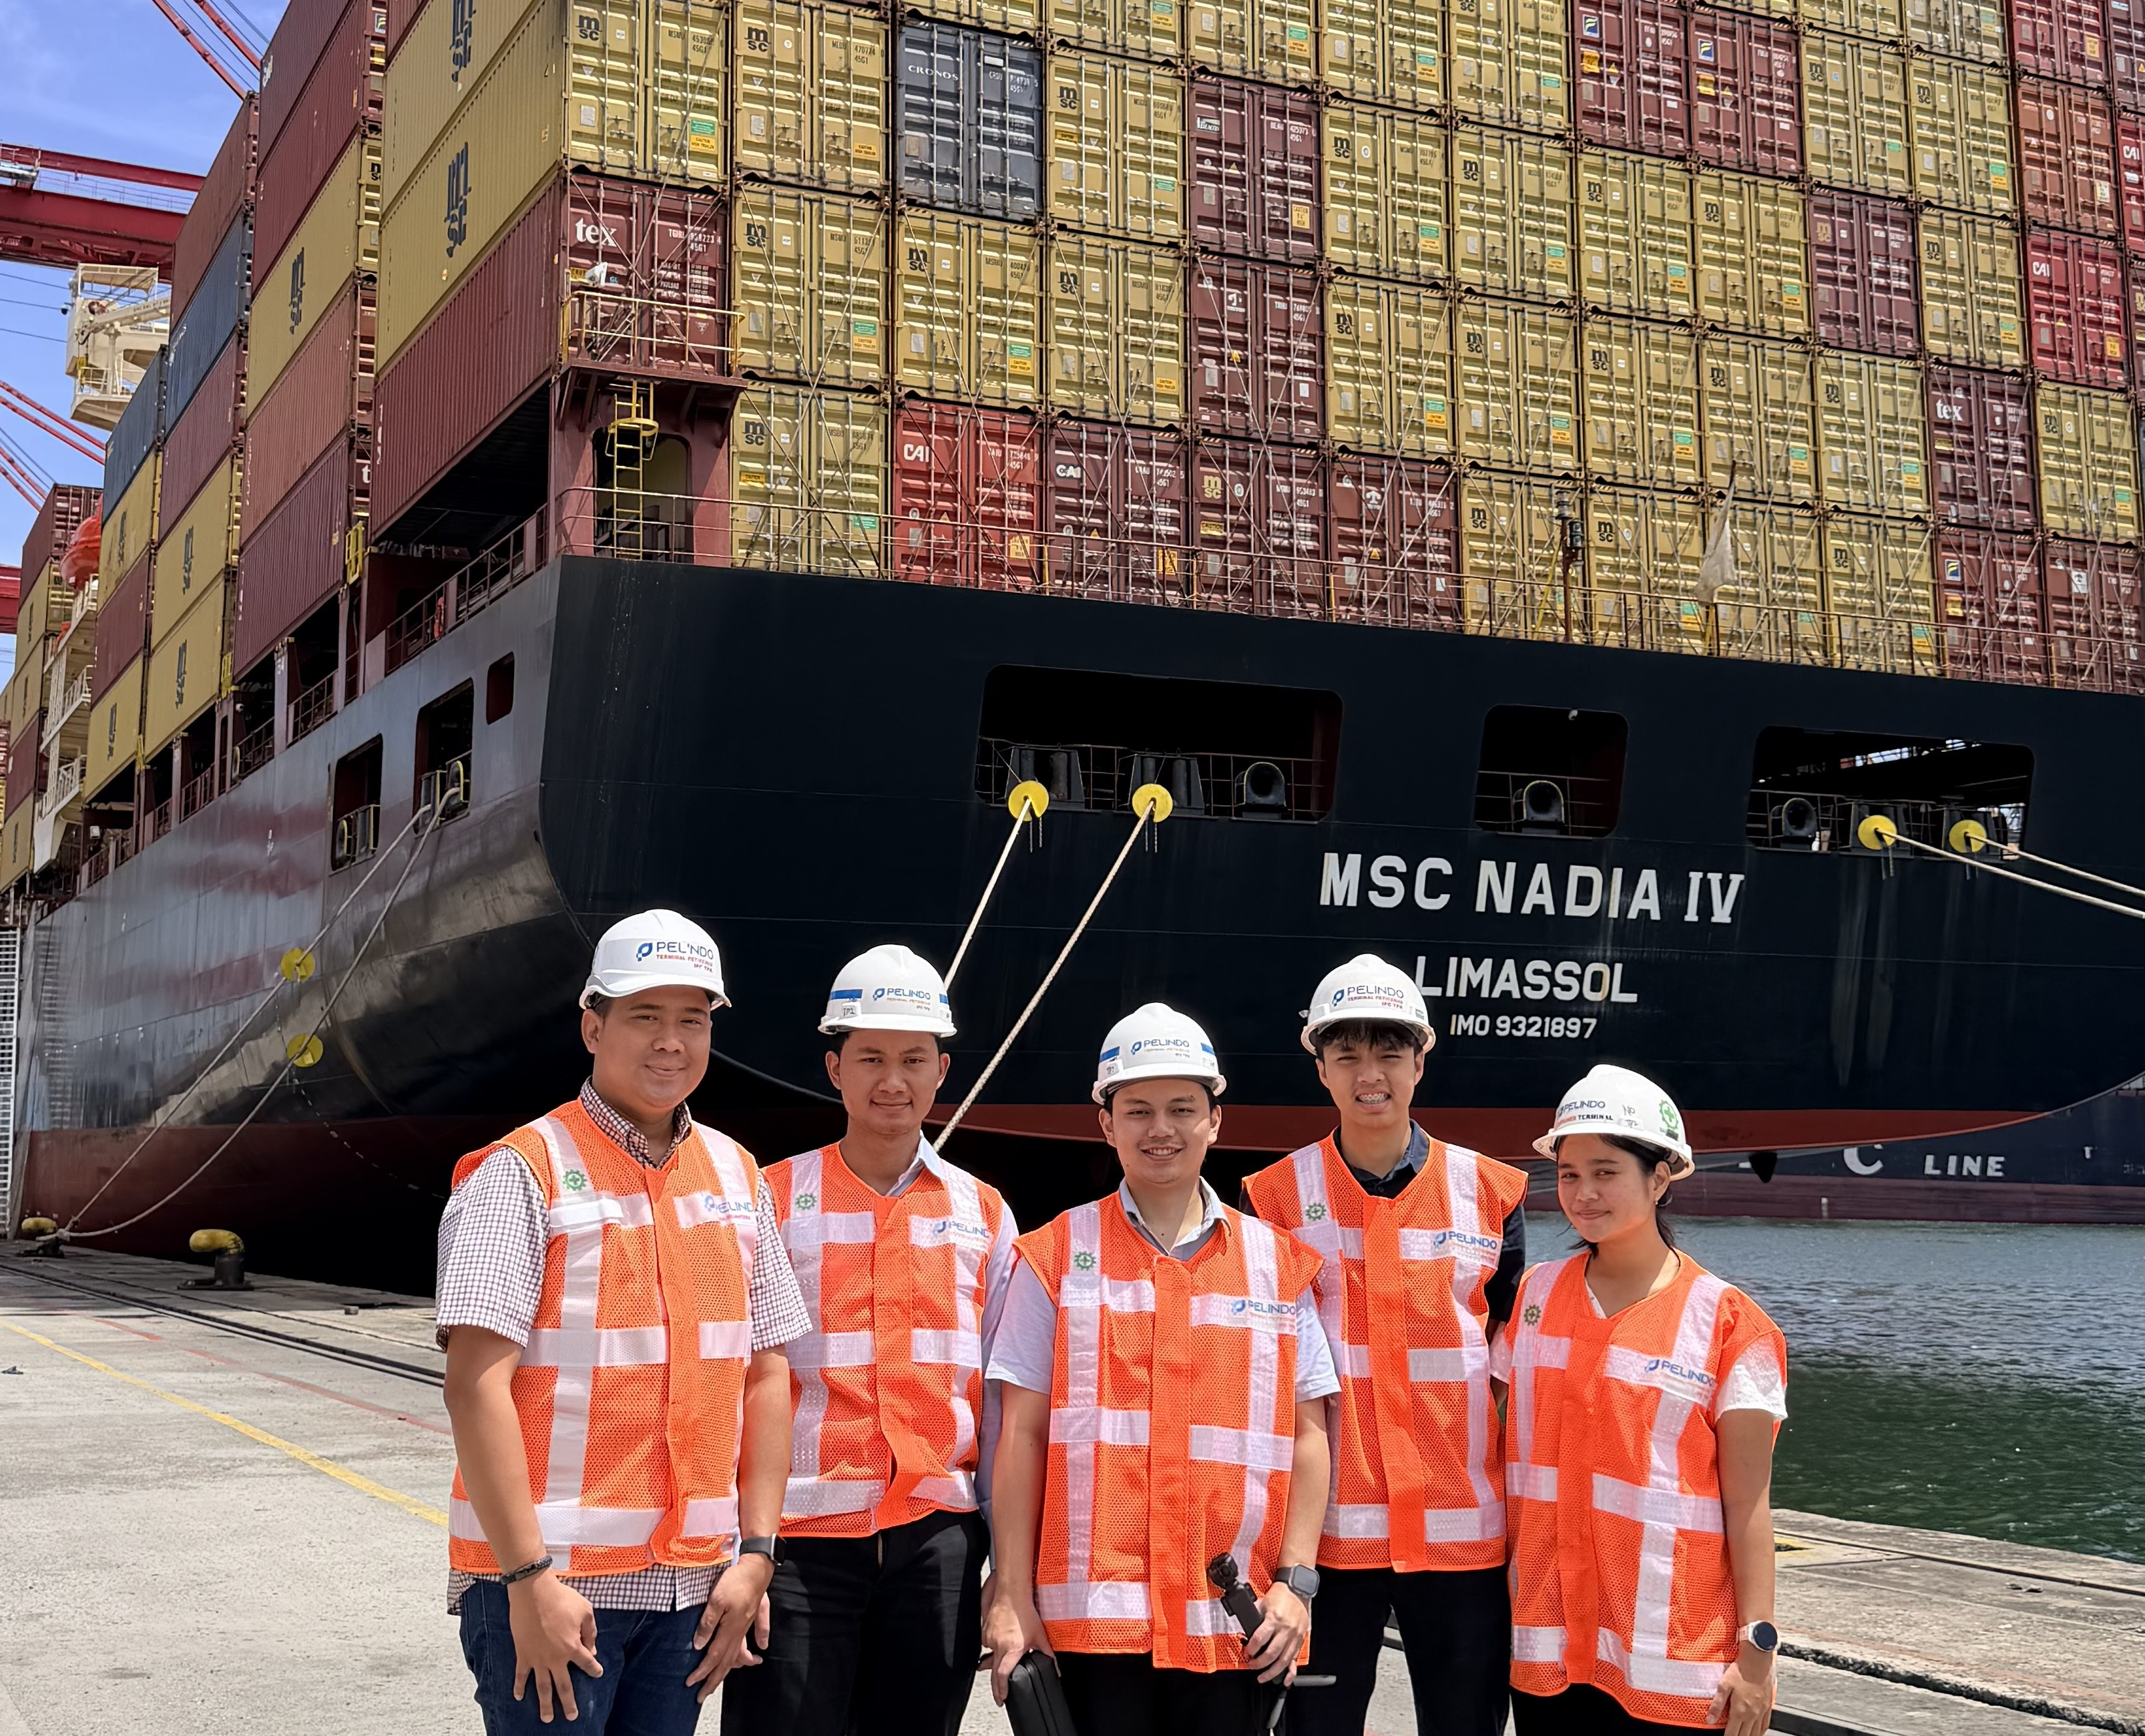
\includegraphics[width=\linewidth]{images/crops/survei-tanjung-priok-tpk-pelindo-crop.jpg}
    \caption{Pelindo}
    \label{fig:survei_tpk_pelindo}
  \end{subfigure}\hfill
  \begin{subfigure}[t]{0.31\textwidth}
    \centering
    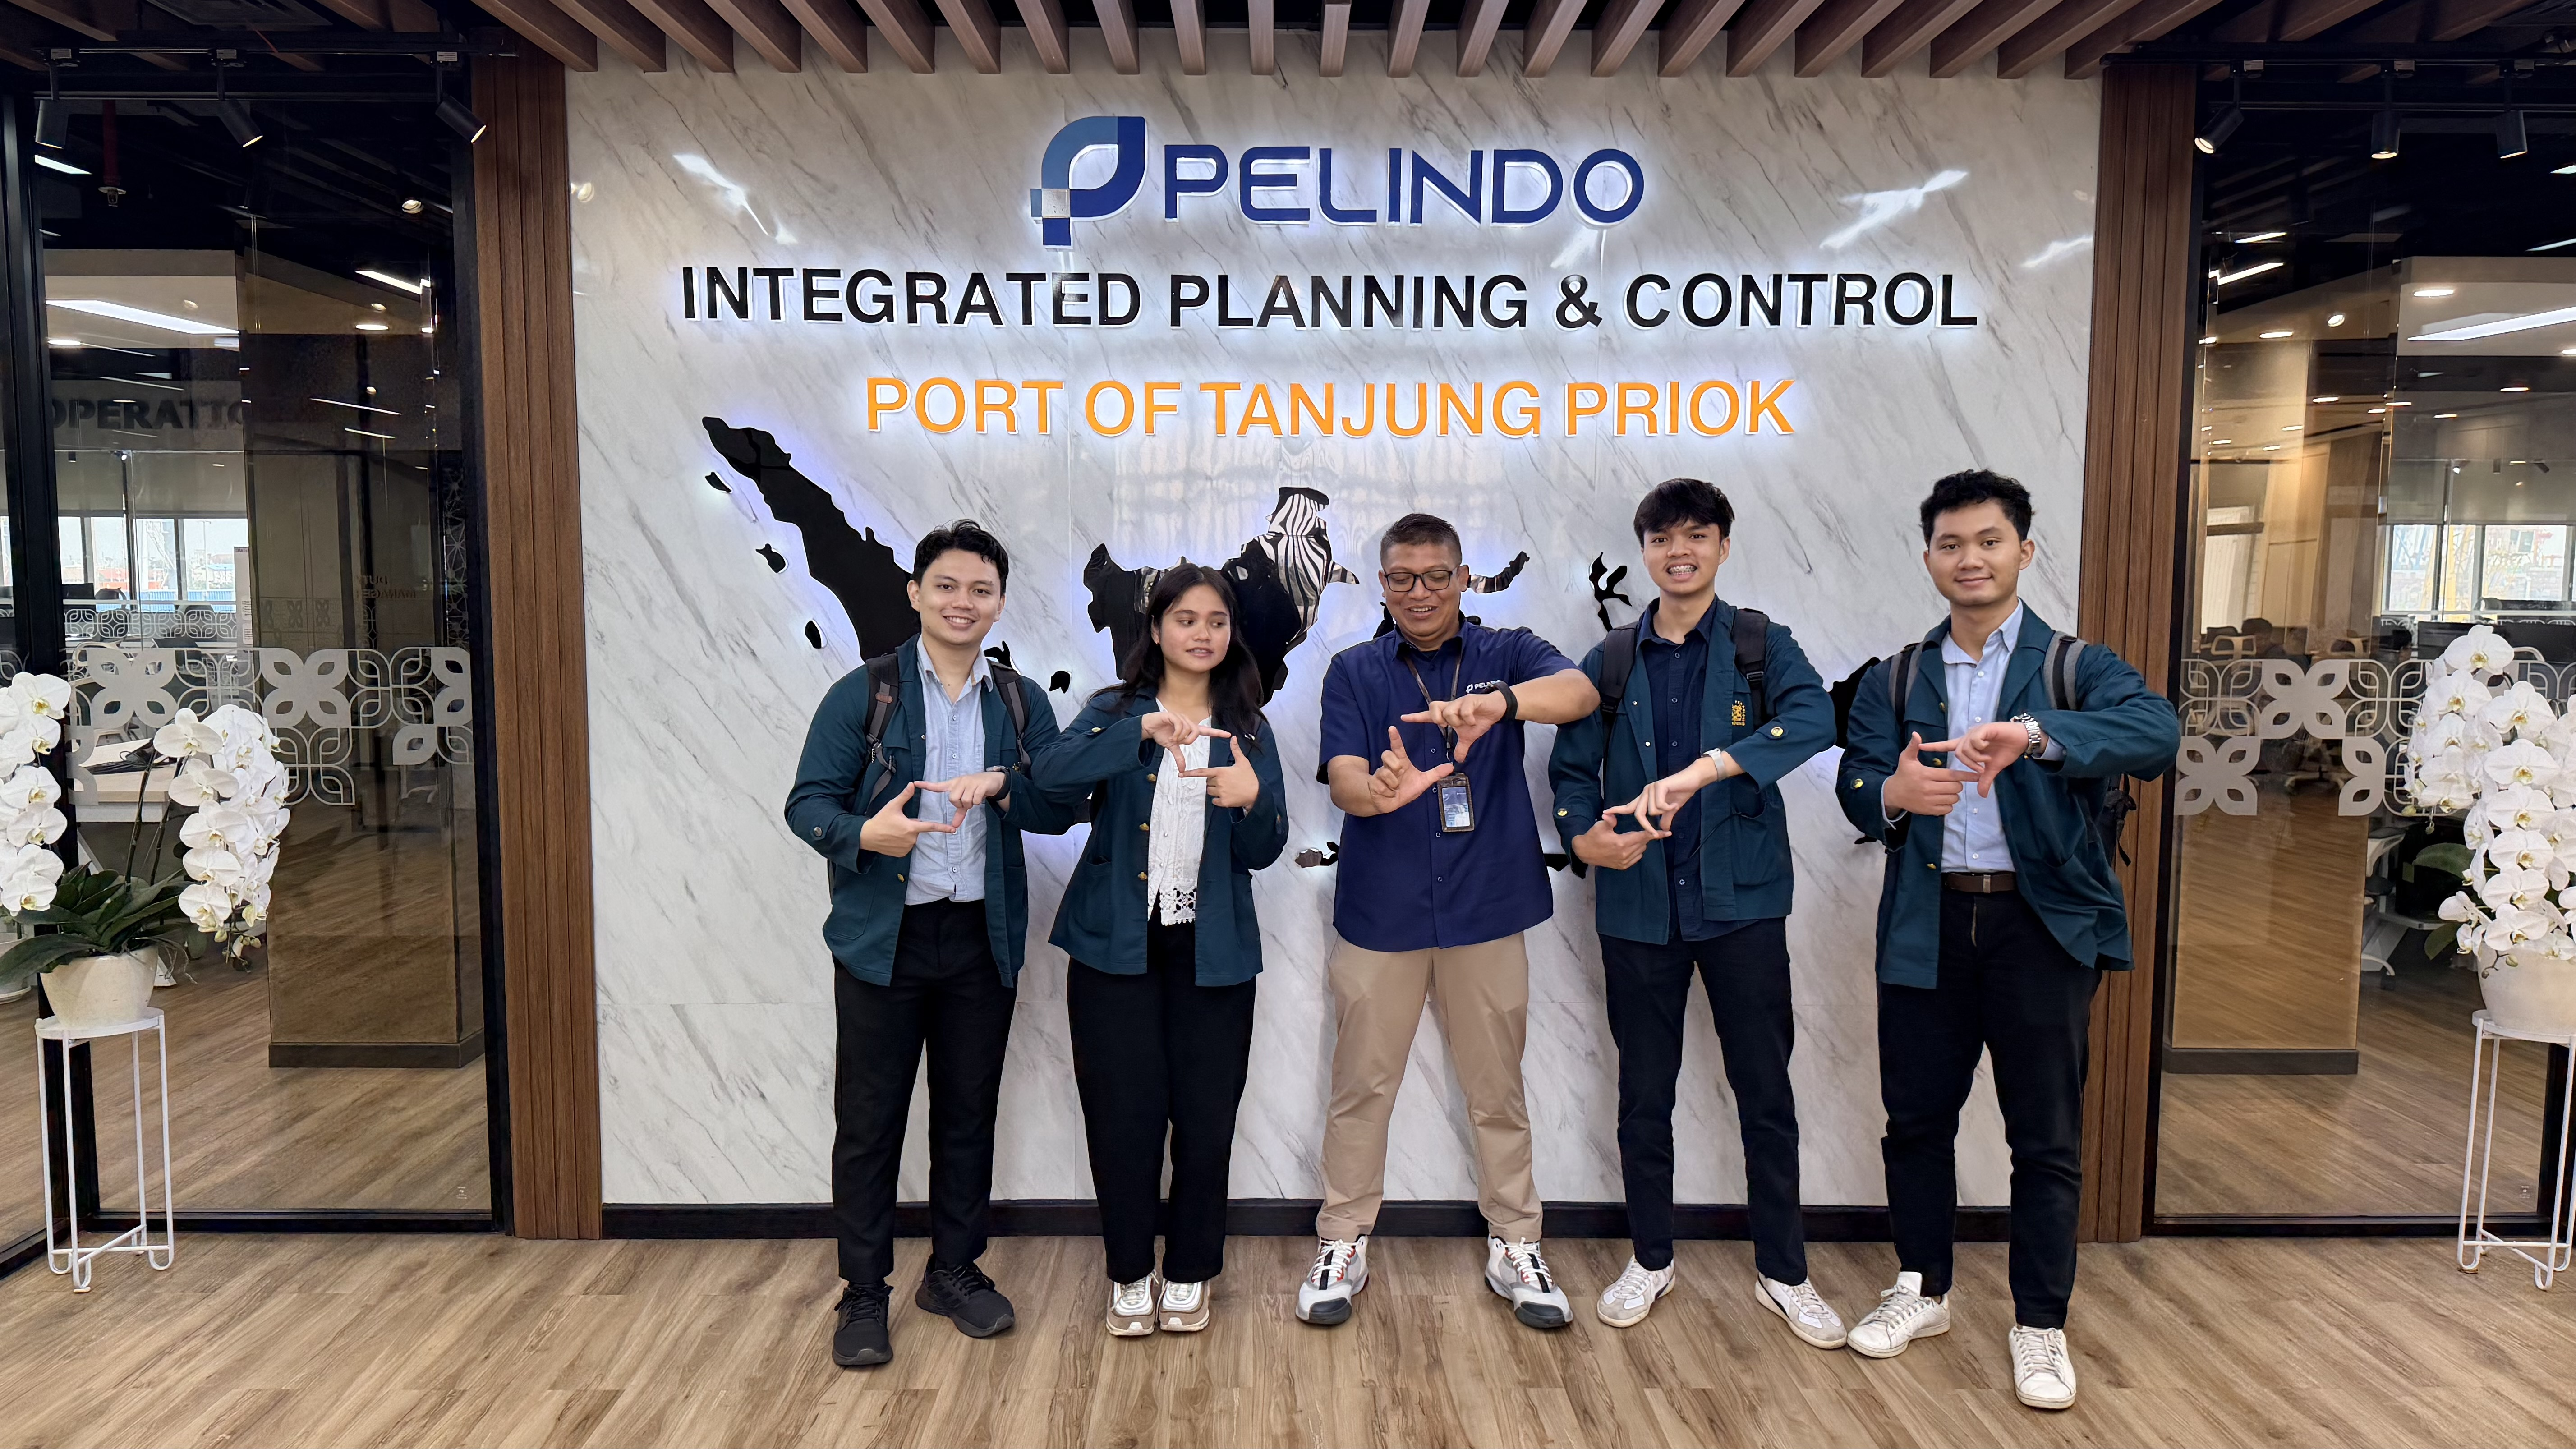
\includegraphics[width=\linewidth]{images/survei-pelindo-2.jpg}
    \caption{Area terminal}
    \label{fig:survei_tpk_pelindo_tambahan_1}
  \end{subfigure}\hfill
  \begin{subfigure}[t]{0.31\textwidth}
    \centering
    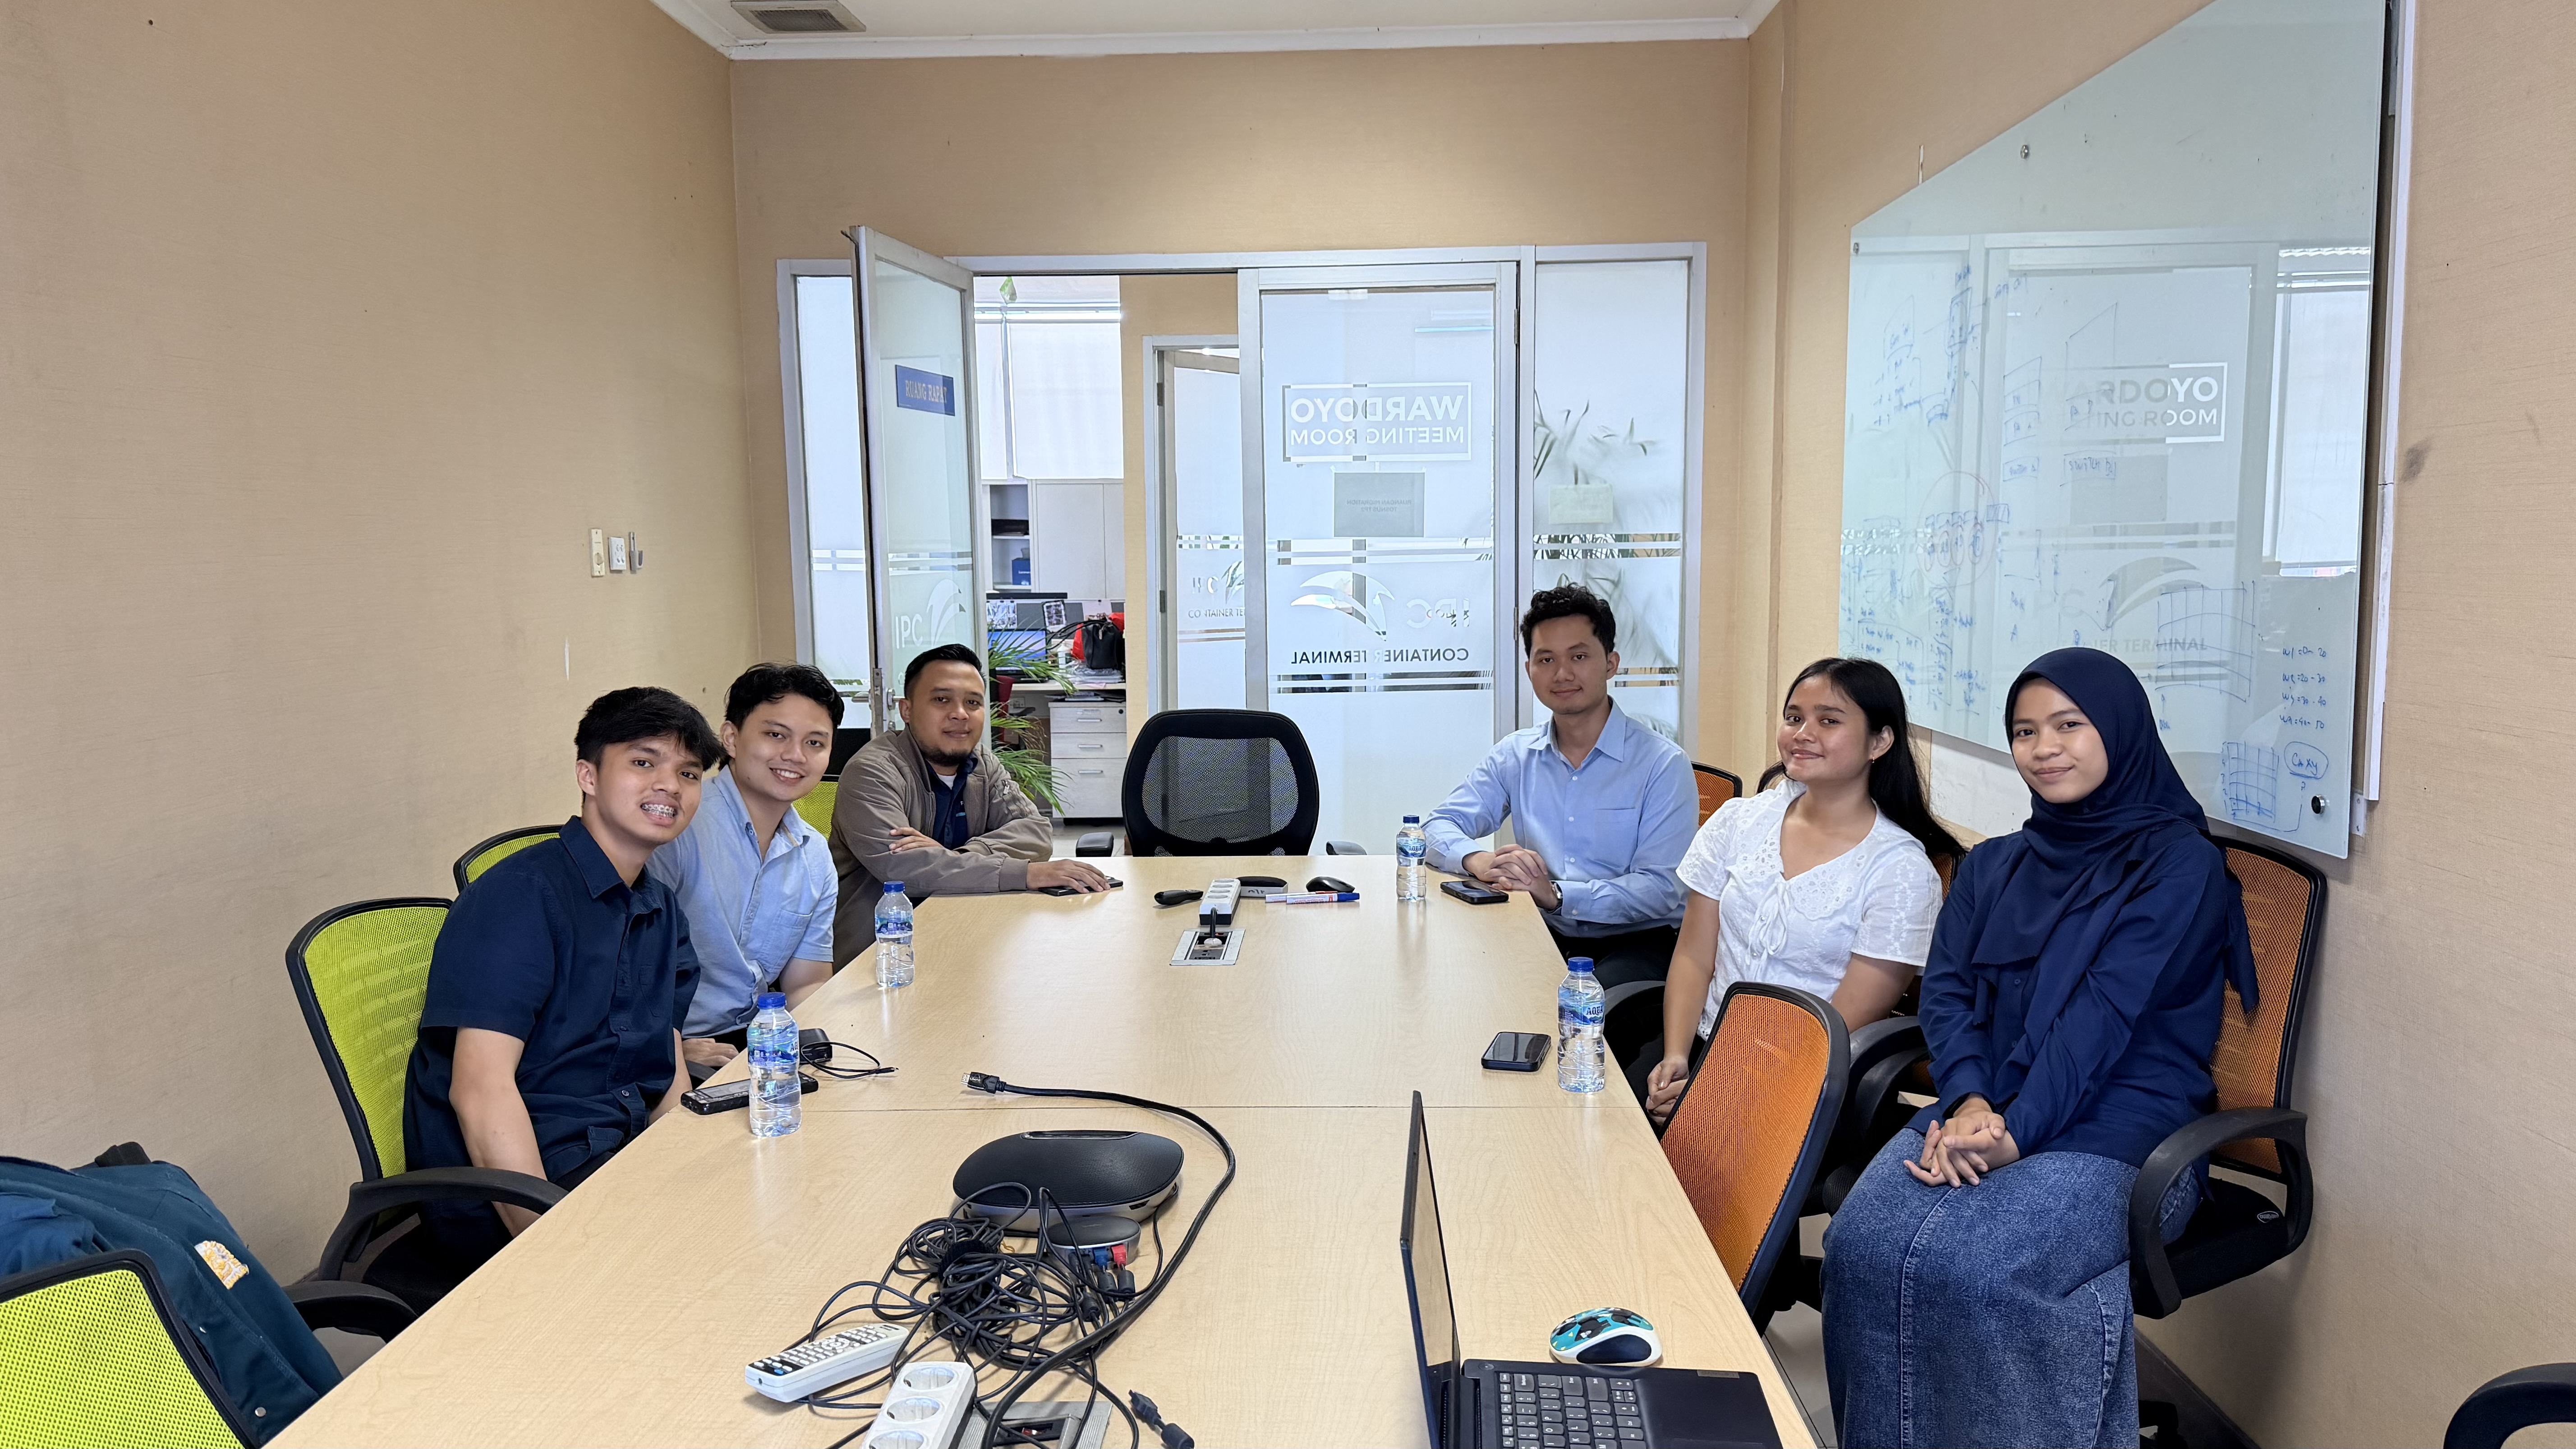
\includegraphics[width=\linewidth]{images/survei-pelindo-3.jpg}
    \caption{Operasional terminal}
    \label{fig:survei_tpk_pelindo_tambahan_2}
  \end{subfigure}

  \vspace{2pt}
  \begin{subfigure}[t]{0.31\textwidth}
    \centering
    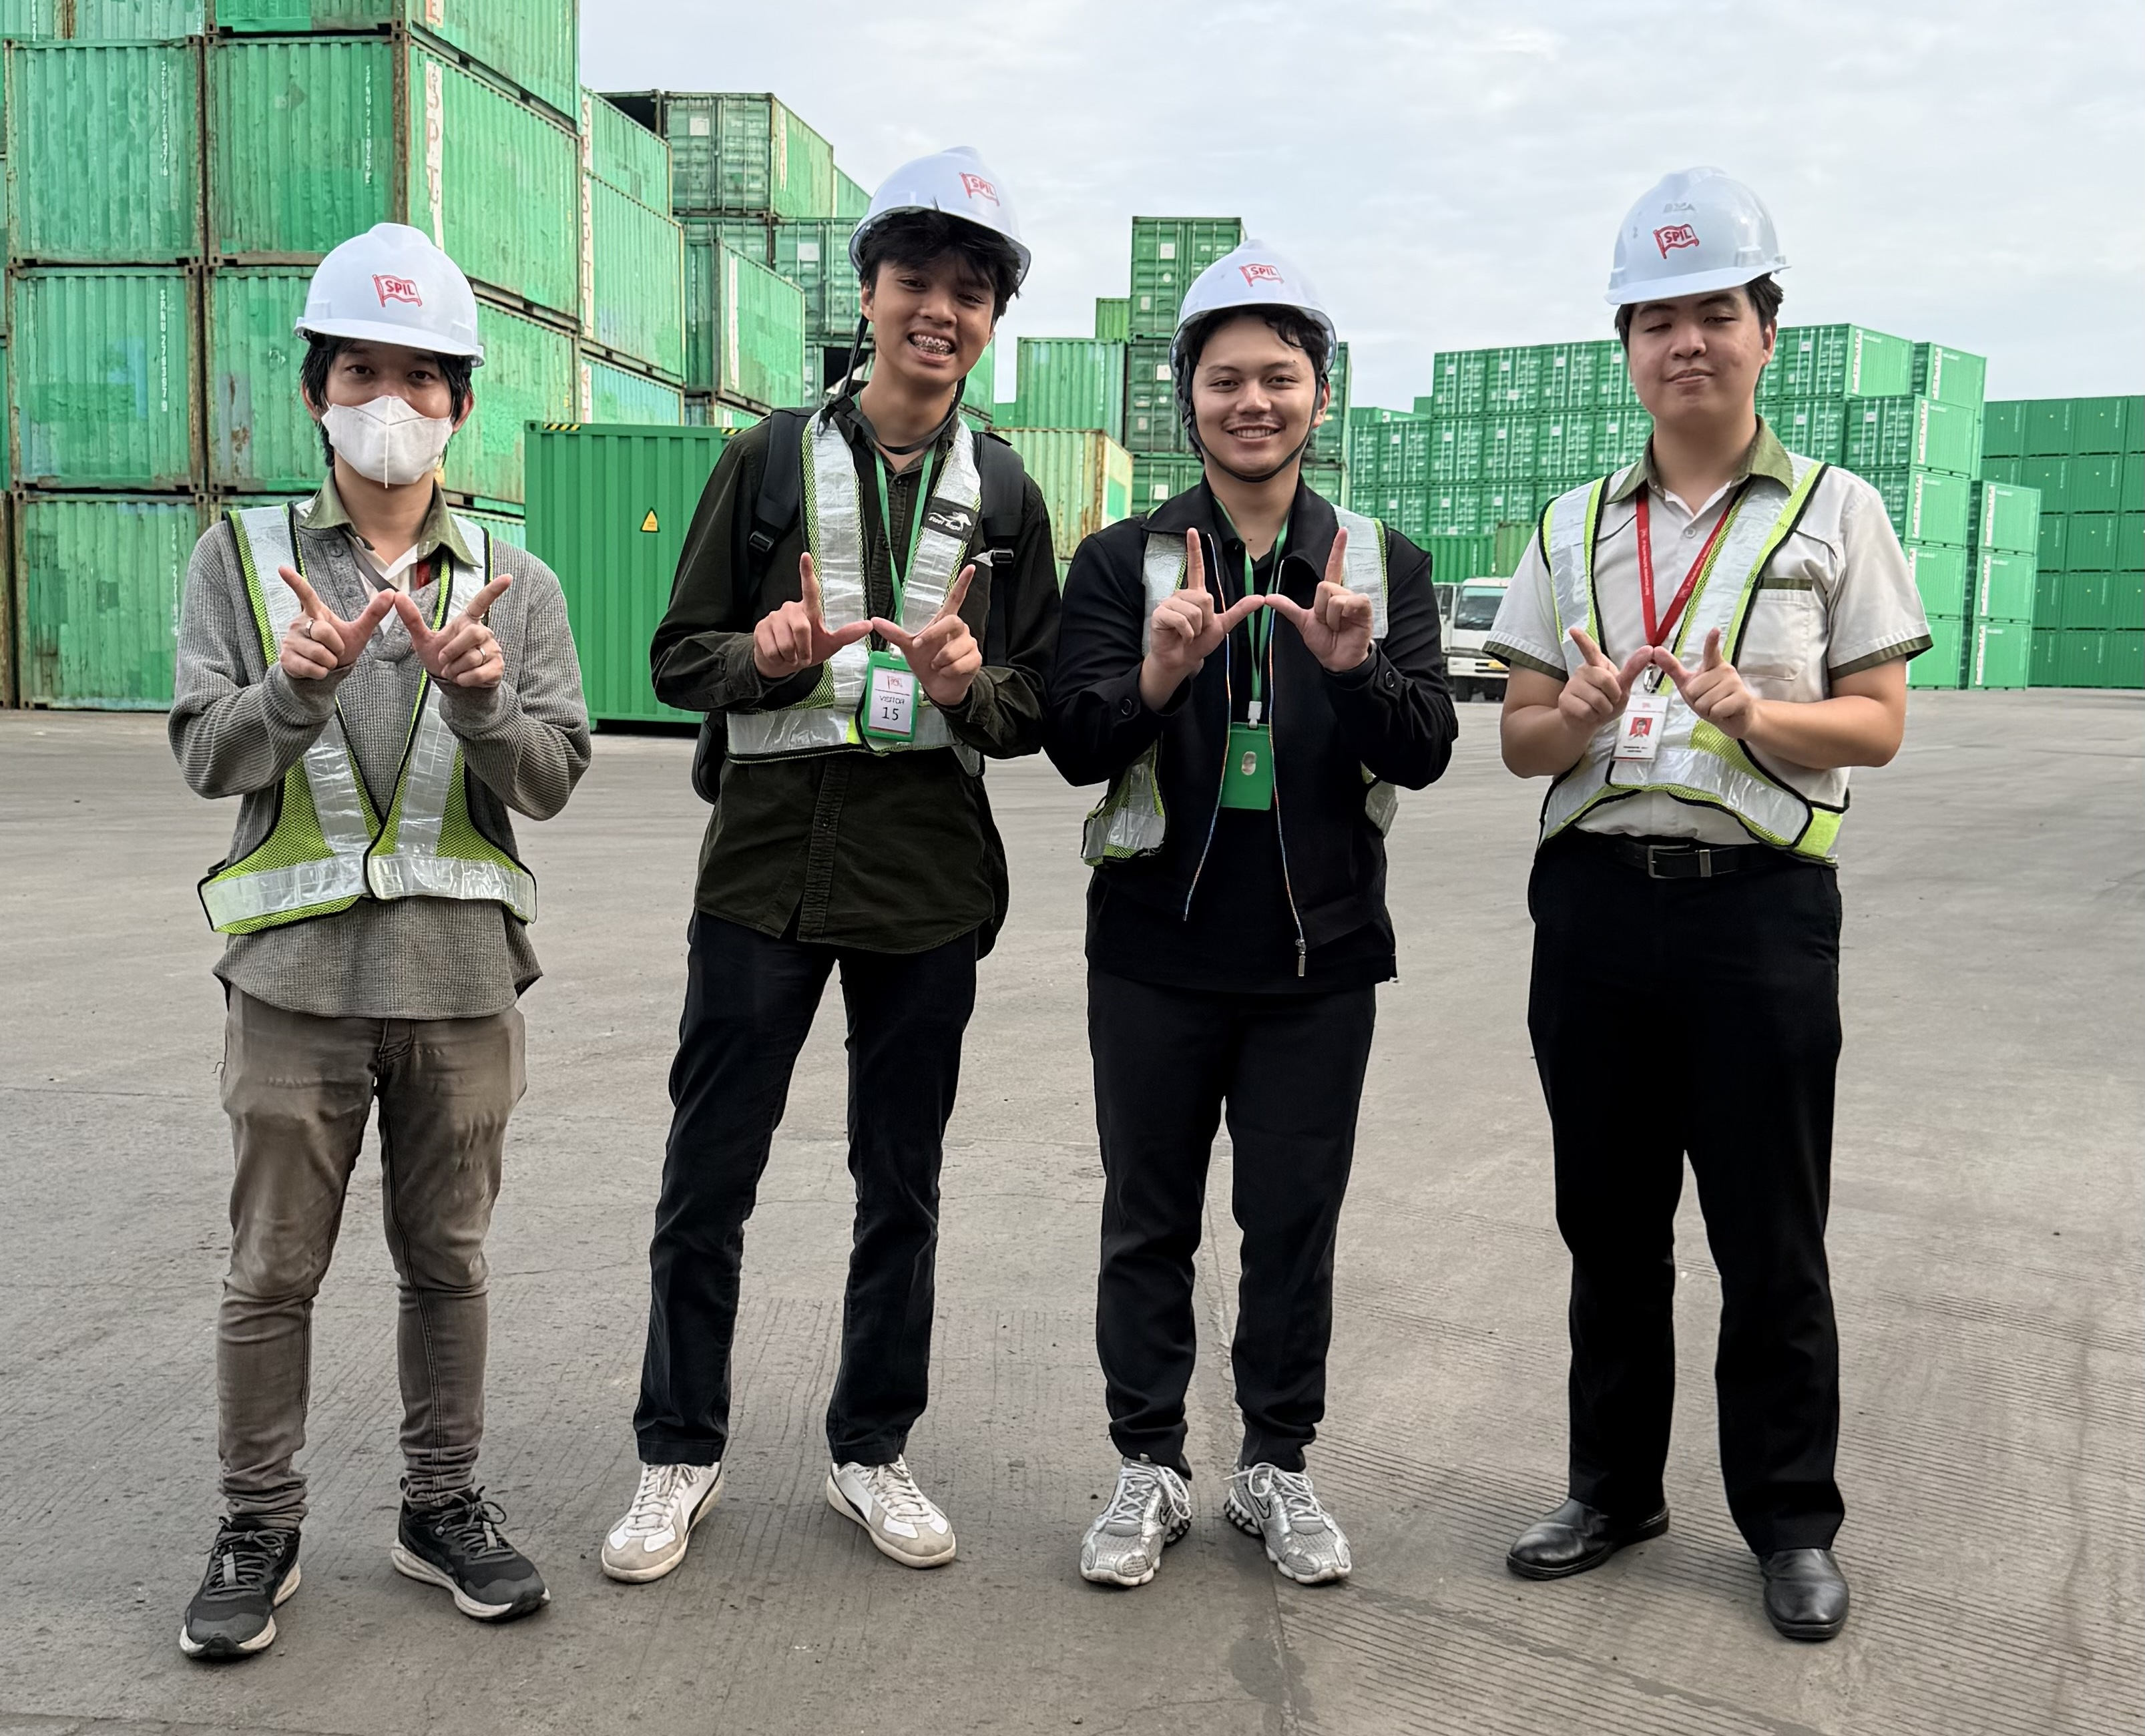
\includegraphics[width=\linewidth]{images/crops/survei-pt-spil-crop.jpg}
    \caption{Depo SPIL}
    \label{fig:survei_pt_spil}
  \end{subfigure}\hspace{0.08\textwidth}
  \begin{subfigure}[t]{0.31\textwidth}
    \centering
    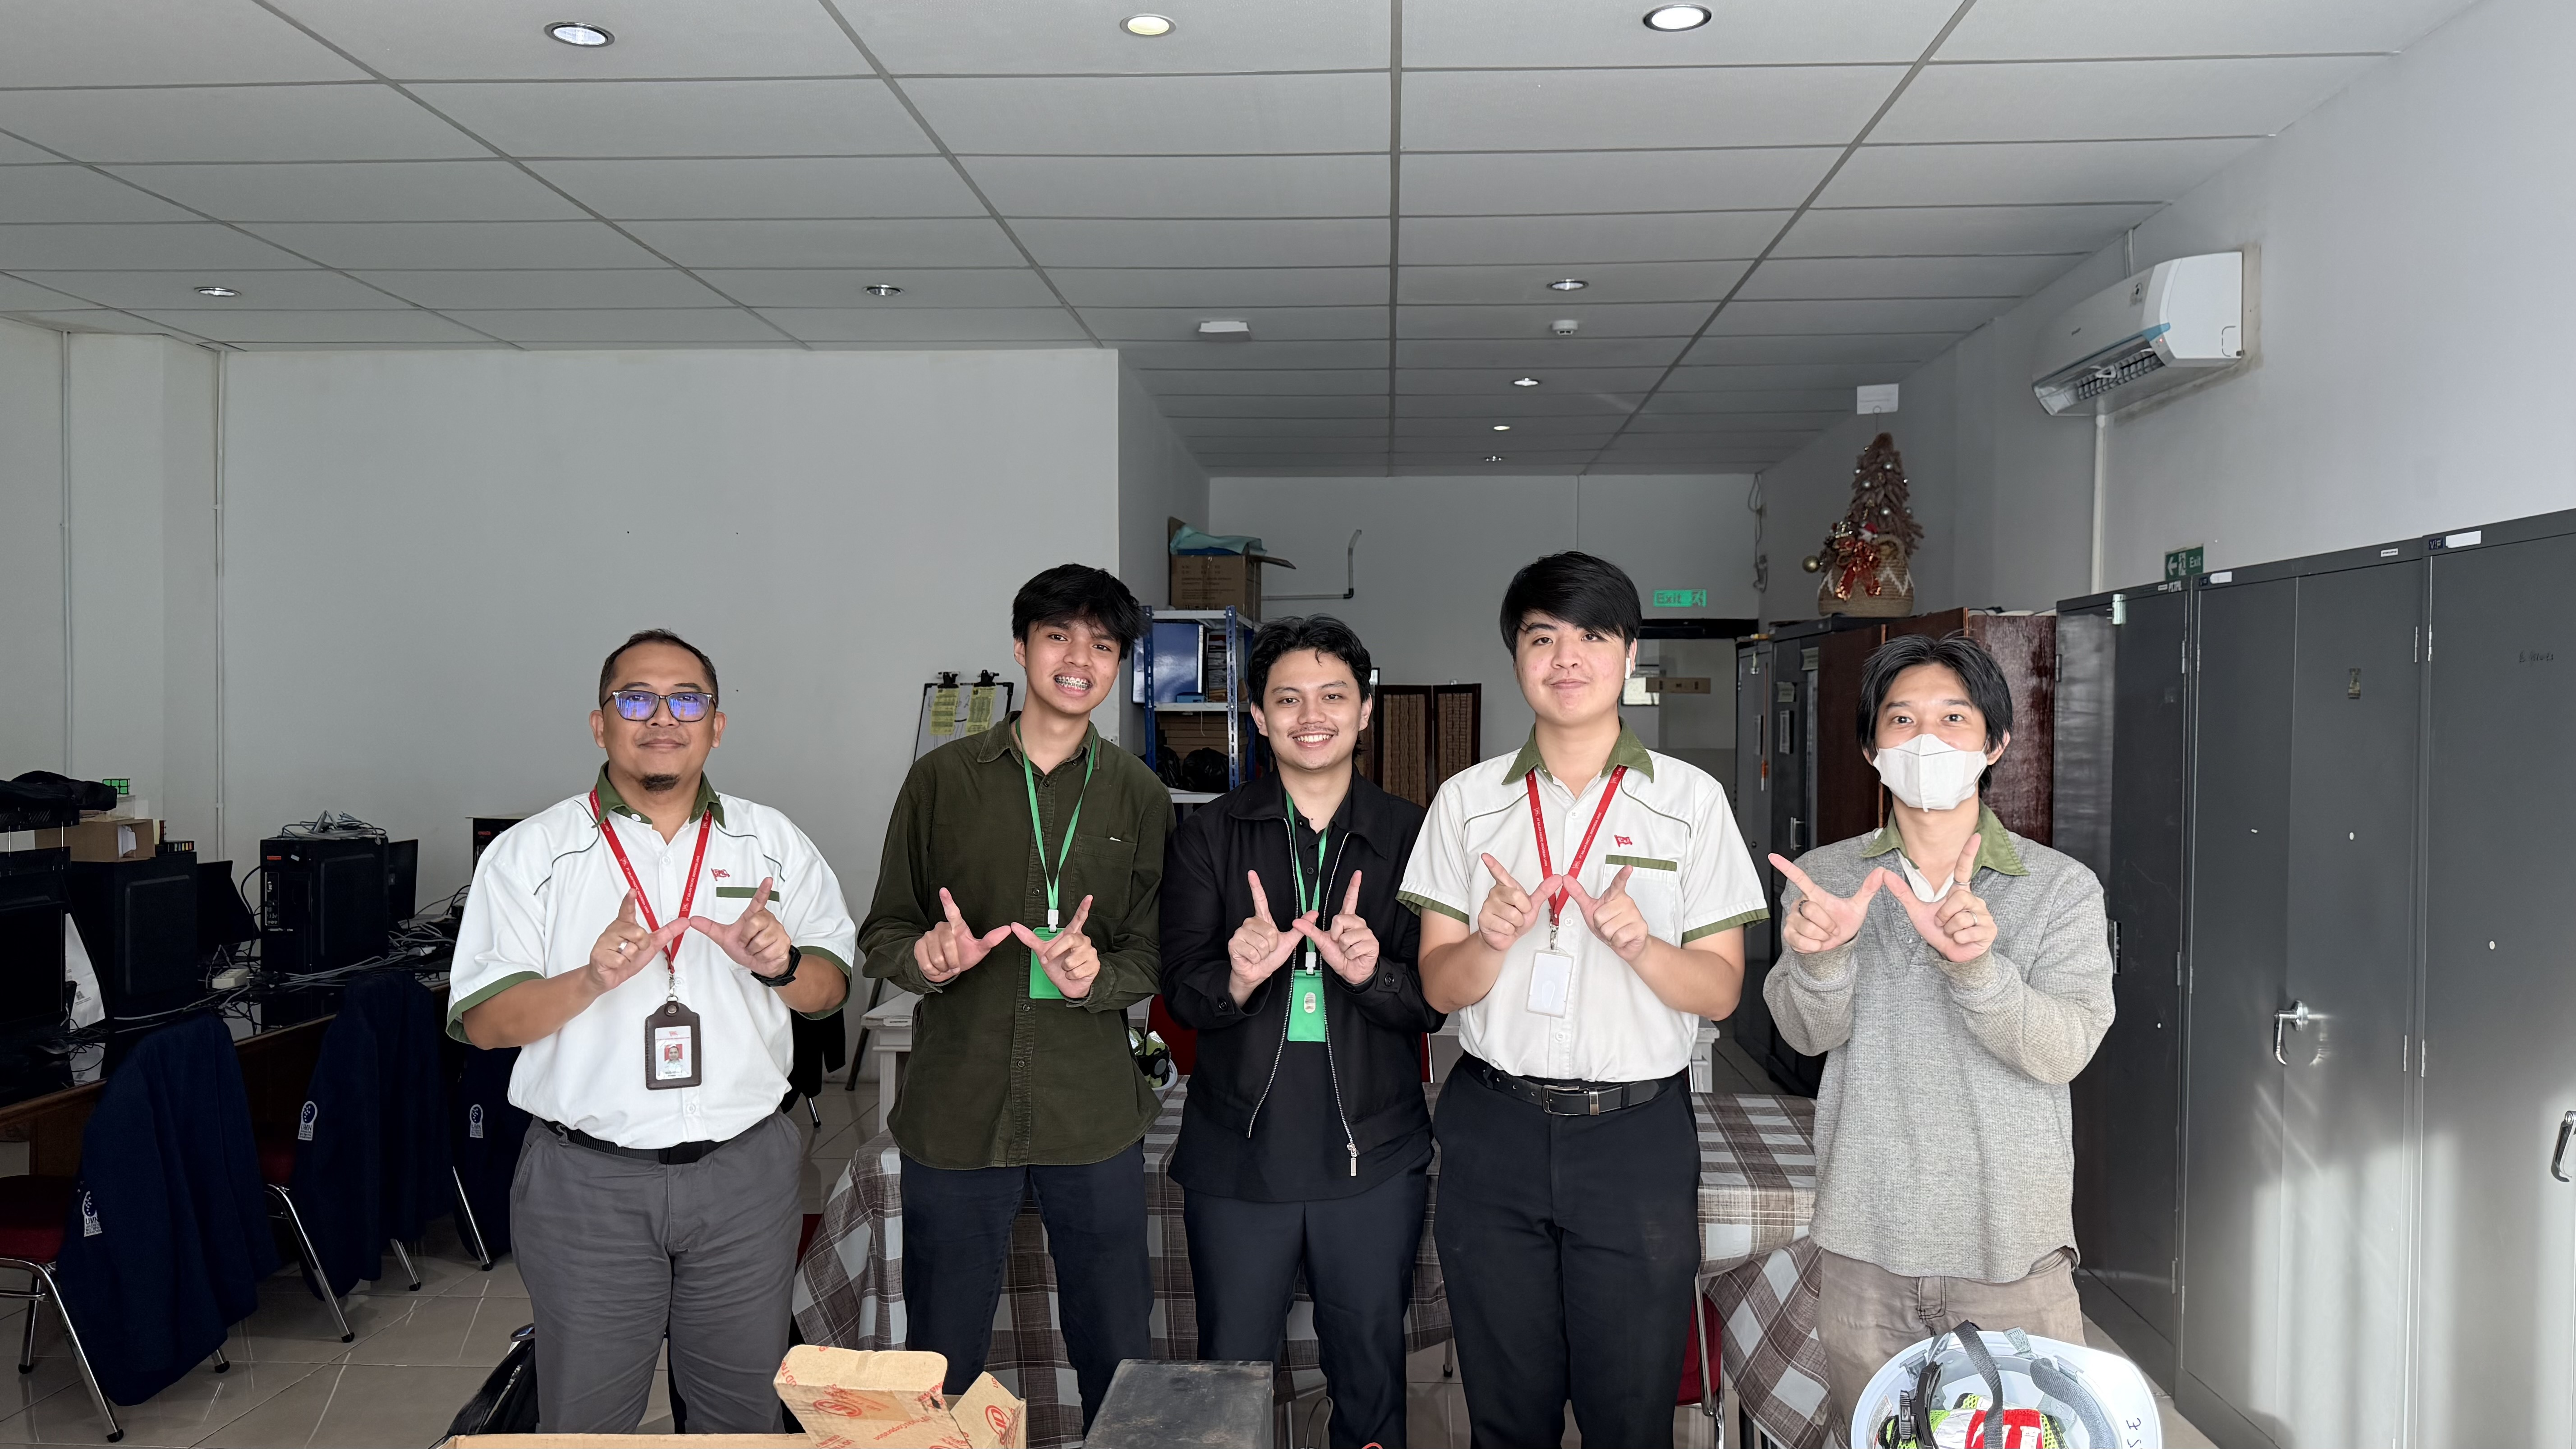
\includegraphics[width=\linewidth]{images/survei-pt-spil-2.jpg}
    \caption{Area depo}
    \label{fig:survei_pt_spil_tambahan}
  \end{subfigure}
  \caption{Ringkasan dokumentasi visual survei lapangan pada Terminal Tanjung Priok Pelindo dan Depo Kontainer Tanjung Priok SPIL}
  \label{fig:ringkasan_dokumentasi_survei}
\end{figure}

Foto pada Gambar~\ref{fig:ringkasan_dokumentasi_survei} digunakan sebagai
arsip konteks lapangan. Bukti kondisi eksisting yang menjadi dasar analisis
utama ditampilkan pada Bab~\ref{chap:analisis-masalah}, sedangkan lampiran ini
berfungsi sebagai dokumentasi pendukung lokasi dan pihak yang diamati.

\section{Ringkasan Temuan Survei dan Dokumen Pendukung}
\label{sec:temuan_survei}
\label{sec:ringkasan_wawancara}

Observasi dan wawancara lapangan digunakan sebagai sumber pendukung untuk
memahami konteks operasional, bukan sebagai transkrip penuh proses bisnis
pelabuhan. Karena sebagian data bersifat terbatas, ringkasan pada lampiran ini
hanya menampilkan tanggal, lokasi, sumber informasi, temuan yang berdampak pada
rancangan arsitektur, dan implikasi perancangannya.

\begin{table}[htbp]
  \centering
  \scriptsize
  \caption{Ringkasan sumber survei lapangan dan implikasi arsitektur}
  \label{tbl:ringkasan-sumber-survei}
  \setlength{\tabcolsep}{3pt}
  \renewcommand{\arraystretch}{1.12}
  \begin{tabularx}{\textwidth}{>{\raggedright\arraybackslash}p{0.15\textwidth} >{\raggedright\arraybackslash}p{0.22\textwidth} >{\raggedright\arraybackslash}X >{\raggedright\arraybackslash}X}
    \toprule
    \textbf{Waktu dan Lokasi} & \textbf{Sumber Informasi} & \textbf{Temuan Ringkas} & \textbf{Implikasi terhadap Rancangan} \\
    \midrule
    3 Februari 2026, Terminal Tanjung Priok Pelindo &
    Observasi area terminal dan wawancara dengan perwakilan operasional, administrasi, serta pemeliharaan sistem informasi &
    Alur terminal sudah memiliki sistem operasional, tetapi pemeriksaan fisik dan pencatatan hasil inspeksi masih membutuhkan koordinasi lintas pihak dan bukti yang dapat ditelusuri. &
    Arsitektur perlu menghubungkan identitas kontainer, hasil inspeksi, bukti visual, dan riwayat proses pada satu entitas kontainer. \\
    26 Februari 2026, Depo Kontainer Tanjung Priok SPIL &
    Observasi depo dan wawancara dengan perwakilan \textit{operational excellence} &
    Informasi kondisi kontainer, status proses, dan bukti visual perlu selaras agar koordinasi antarunit kerja tidak bergantung pada catatan terpisah. &
    Sistem perlu menyediakan struktur data yang konsisten dan antarmuka yang menampilkan riwayat kontainer secara ringkas. \\
    Dokumen pendukung layanan \textit{screening} dan tata kelola TI &
    Pedoman tata kelola TI, alur proses \textit{screening}, SLA/BCP pemindai, diagram integrasi, dan prosedur insiden &
    Layanan inspeksi dan \textit{screening} berada dalam konteks formal yang melibatkan integrasi sistem, kontrol akses, keberlangsungan layanan, dan penanganan insiden. &
    Rancangan perlu memisahkan tanggung jawab komponen, menyiapkan pola integrasi, dan menyediakan jejak audit serta bukti inspeksi. \\
    \bottomrule
  \end{tabularx}
\end{table}

\FloatBarrier

\section{Bukti Tampilan Realisasi Sistem}
\label{sec:bukti_tampilan_realisasi}

Bagian ini memuat contoh tampilan antarmuka sistem yang digunakan sebagai bukti
visual pendukung pada evaluasi arsitektur. Bukti ini tidak ditujukan untuk
menilai kualitas antarmuka secara rinci, melainkan untuk menunjukkan bahwa
keputusan arsitektural yang dibahas pada Bab~\ref{chap:evaluasi} memang telah
direalisasikan dalam bentuk alur sistem yang dapat diamati.

\begin{figure}[htbp]
  \centering
  \begin{subfigure}[t]{0.32\textwidth}
    \centering
    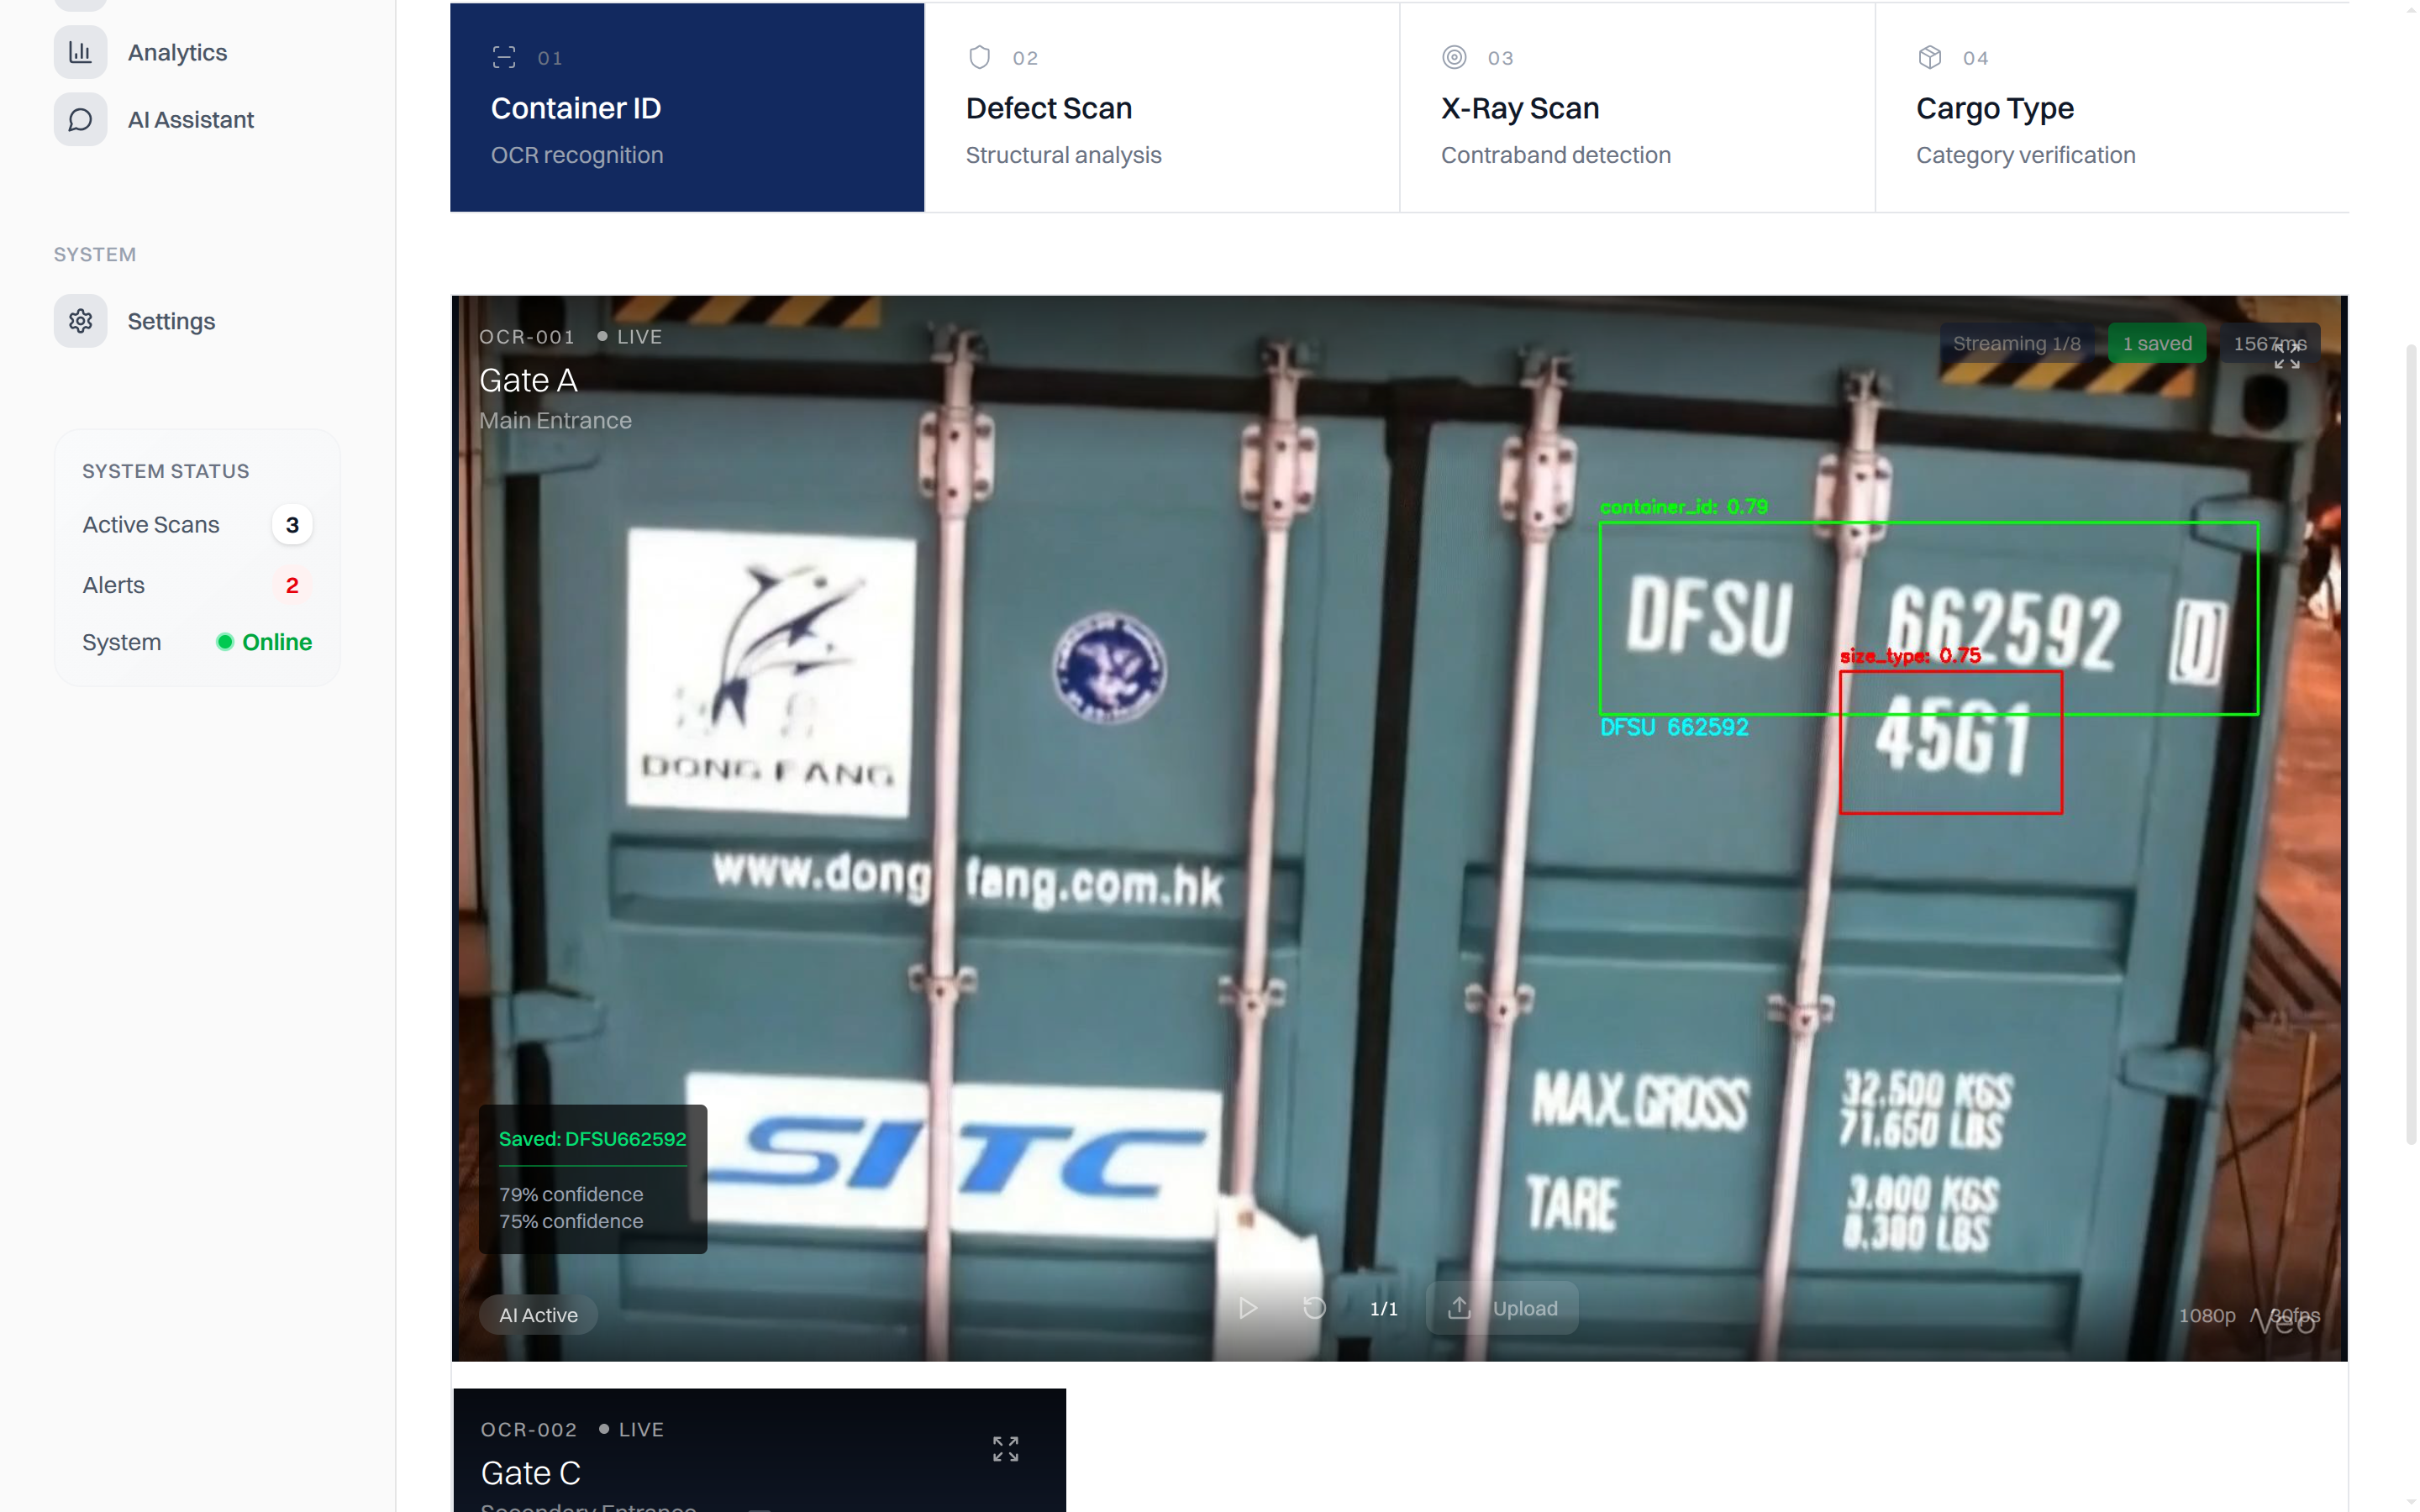
\includegraphics[width=\linewidth]{images/evidence-ocr-live.png}
    \caption{Aliran OCR}
    \label{fig:evidence_ocr_live}
  \end{subfigure}\hfill
  \begin{subfigure}[t]{0.32\textwidth}
    \centering
    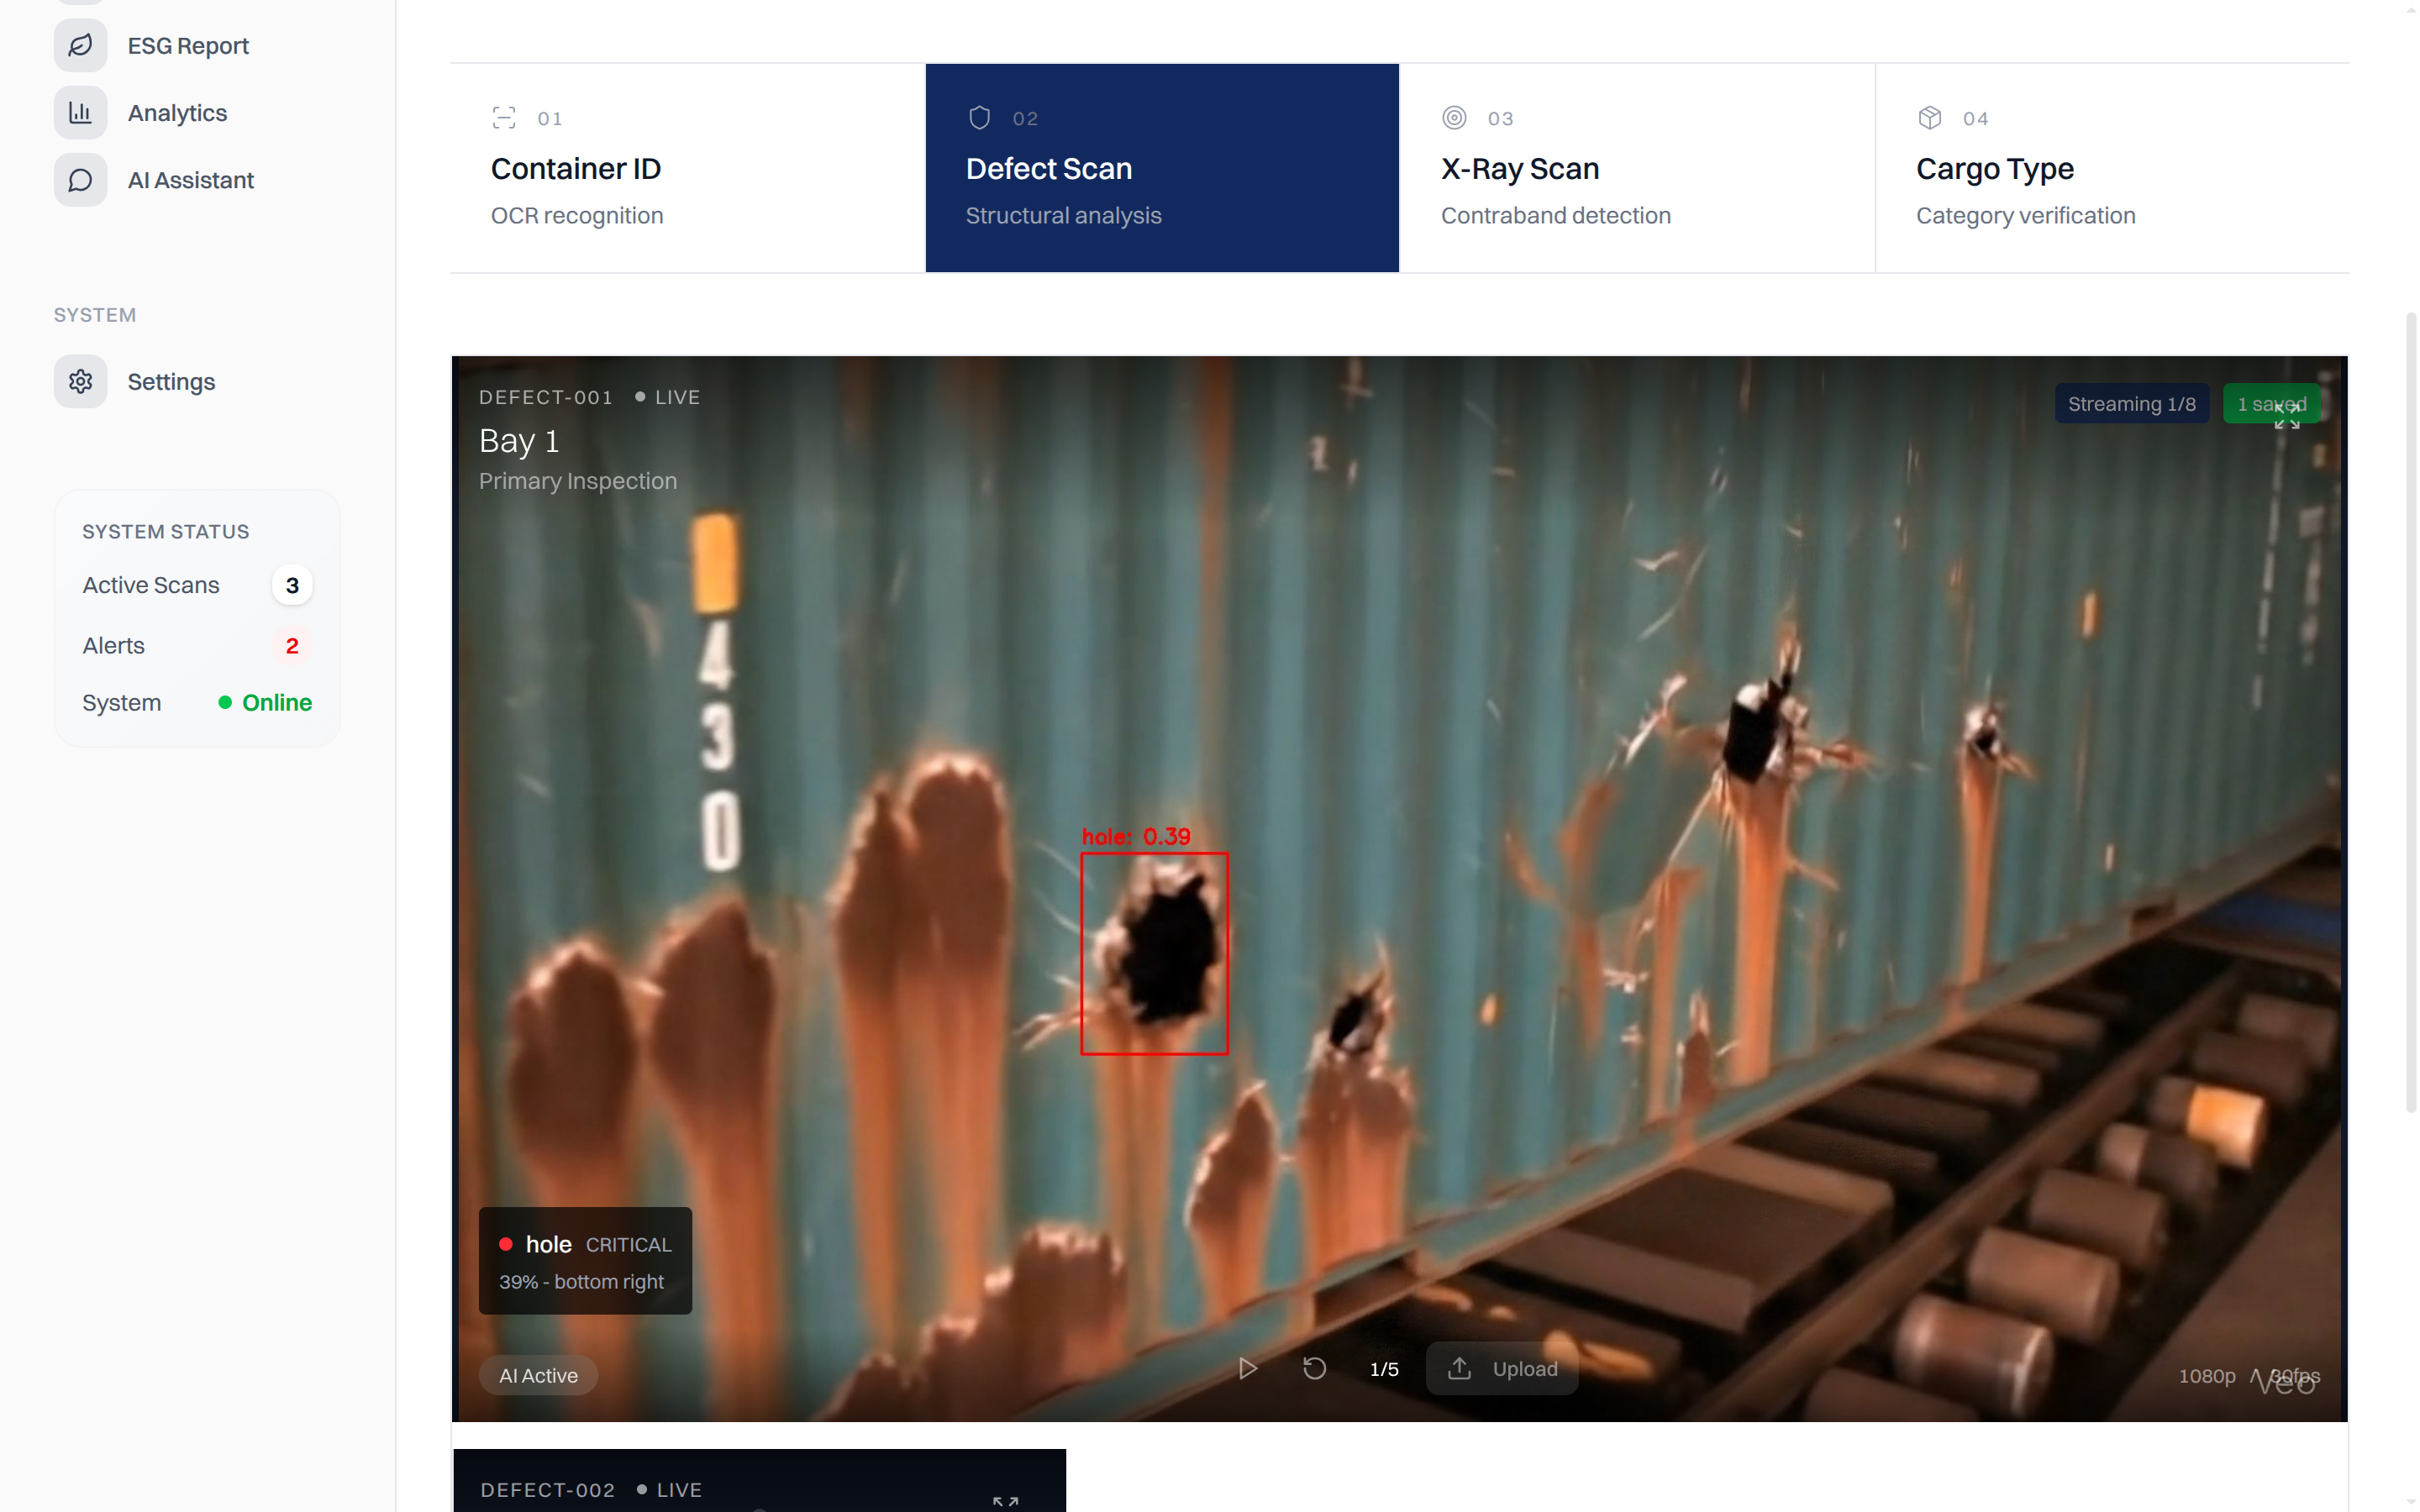
\includegraphics[width=\linewidth]{images/evidence-defect-live.png}
    \caption{\textit{Defect scan}}
    \label{fig:evidence_defect_live}
  \end{subfigure}\hfill
  \begin{subfigure}[t]{0.32\textwidth}
    \centering
    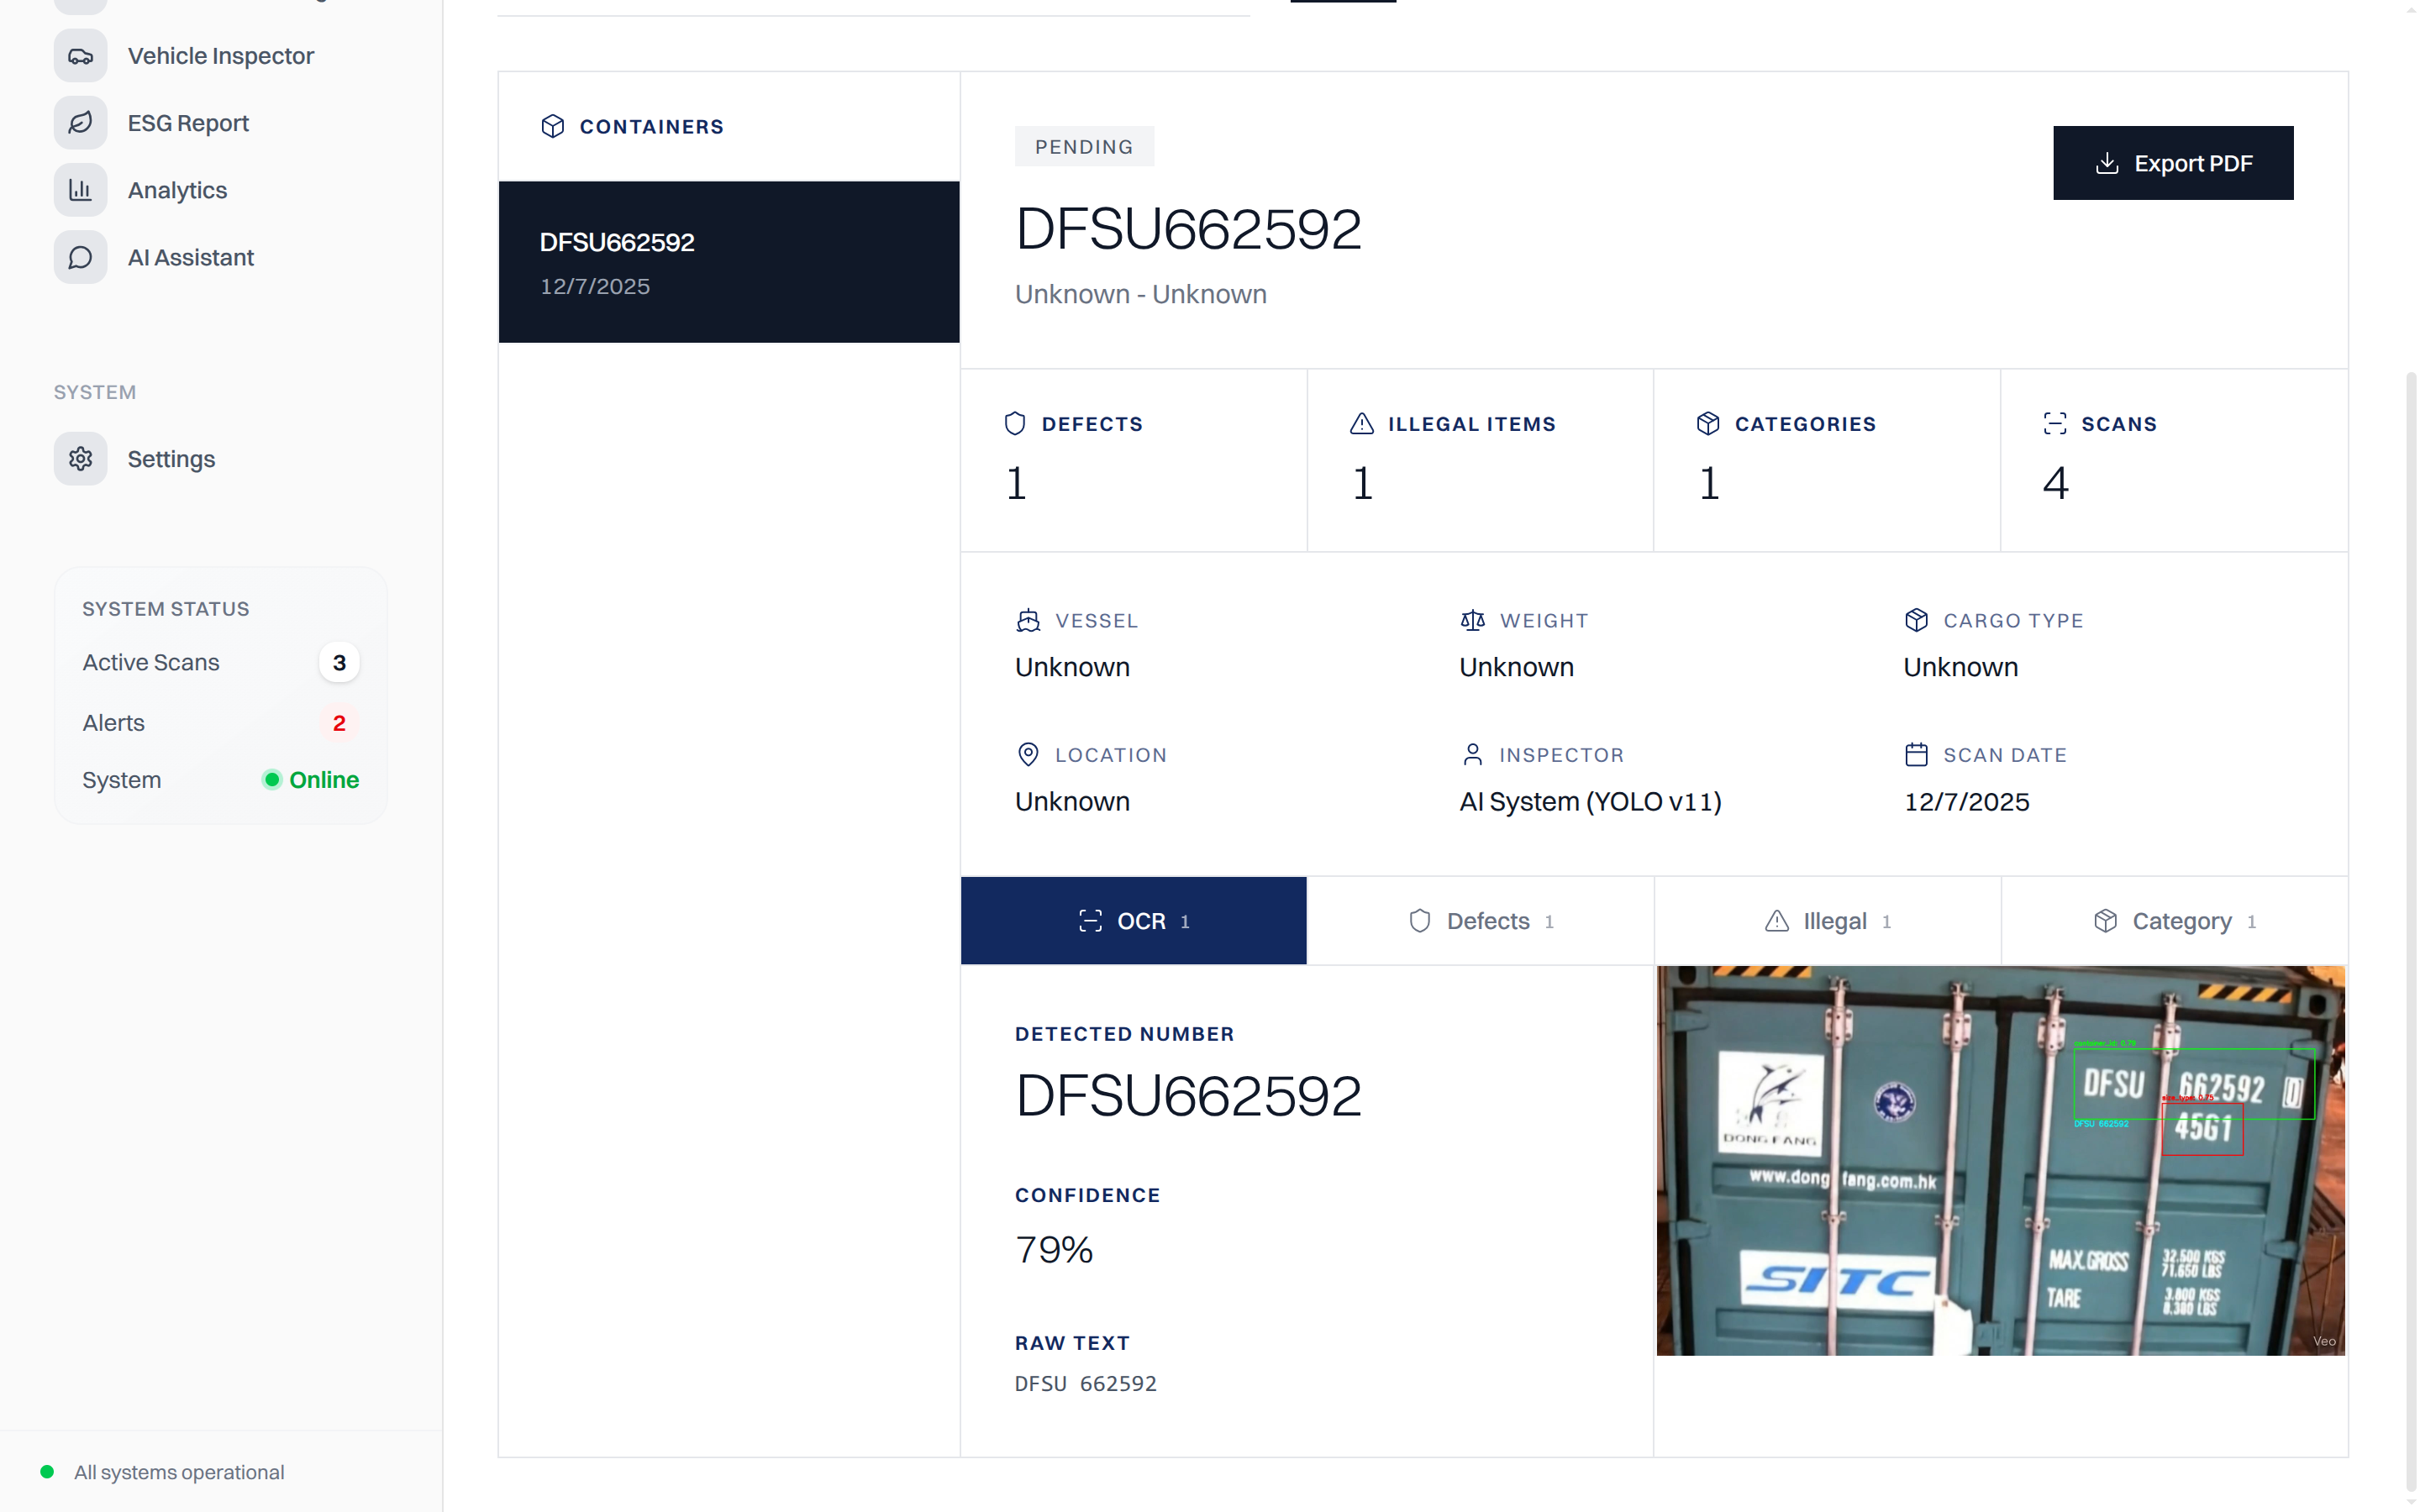
\includegraphics[width=\linewidth]{images/evidence-container-detail.png}
    \caption{Detail kontainer}
    \label{fig:evidence_container_detail}
  \end{subfigure}
  \caption{Ringkasan bukti tampilan realisasi sistem pada alur OCR, pemindaian kerusakan, dan detail kontainer}
  \label{fig:evidence_realisasi_sistem_ringkas}
\end{figure}

Ketiga tampilan tersebut mendukung tiga pembuktian utama. Pertama, nomor
kontainer dapat dikenali dari aliran OCR dan digunakan sebagai identitas objek
inspeksi. Kedua, hasil pemindaian kerusakan dapat ditampilkan langsung pada
jalur video terpisah dari data transaksional. Ketiga, hasil dari beberapa
proses inspeksi dapat disajikan kembali pada satu halaman detail kontainer,
sehingga keputusan arsitektural mengenai integrasi data, pemisahan jalur
komunikasi, serta riwayat kontainer memiliki bukti realisasi yang dapat
diamati secara langsung.

\section{Contoh Struktur Data Inti dan Penyimpanan Artefak}
\label{sec:contoh-struktur-data}

Selain bukti tampilan antarmuka, evaluasi arsitektur juga diperkuat dengan
contoh struktur data inti yang digunakan sistem. Contoh ini menunjukkan bahwa
hasil OCR, hasil pemindaian kerusakan, hasil pemindaian barang berisiko, hasil
klasifikasi muatan, hasil tinjauan manual, dan lampiran bukti visual memang
terkonsolidasi pada satu entitas kontainer. Demi menjaga kerahasiaan, sebagian
nilai identitas pengguna disamarkan tanpa mengubah struktur data utamanya.

\begin{lstlisting}[language={}, numbers=none, basicstyle=\ttfamily\scriptsize, breaklines=true, caption={Cuplikan struktur data inti pada entitas kontainer}, label=lst:container-entity-sample]
{
  "containerNumber": "DFSU6625920",
  "userEmail": "<disamarkan>",
  "ocr": {
    "detectedNumber": "DFSU6625920",
    "confidence": 0.79,
    "status": "SUCCESS"
  },
  "manifest": {
    "found": false,
    "source": "NOT_FOUND"
  },
  "defectScan": {
    "summary": {
      "total": 1,
      "critical": 1
    },
    "hasCriticalDefects": true,
    "status": "SUCCESS"
  },
  "illegalScan": {
    "hasIllegalItems": true,
    "threatLevel": "NONE",
    "status": "SUCCESS"
  },
  "categoryScan": {
    "detectedCategories": ["Spare_Part"],
    "matchesManifest": false,
    "status": "SUCCESS"
  },
  "manualReview": {
    "required": true,
    "reviewed": true,
    "decision": "APPROVE"
  },
  "attachments": [
    {
      "type": "PHOTO",
      "source": "MOBILE_APP",
      "url": "https://cdn.cargovision.app/evidence/<container-id>/<file>.jpg"
    }
  ],
  "status": "CLEARED"
}
\end{lstlisting}

Cuplikan pada Listing~\ref{lst:container-entity-sample} memperlihatkan bahwa
nomor kontainer berfungsi sebagai jangkar integrasi, sedangkan hasil-hasil
inspeksi disimpan pada bidang-bidang terstruktur di dalam entitas yang sama.
Struktur ini mendukung argumen bahwa arsitektur data yang dirancang memang
memungkinkan penggabungan konteks OCR, kerusakan, barang berisiko, klasifikasi
muatan, tinjauan manual, dan lampiran bukti visual secara konsisten.

\begin{figure}[htbp]
  \centering
  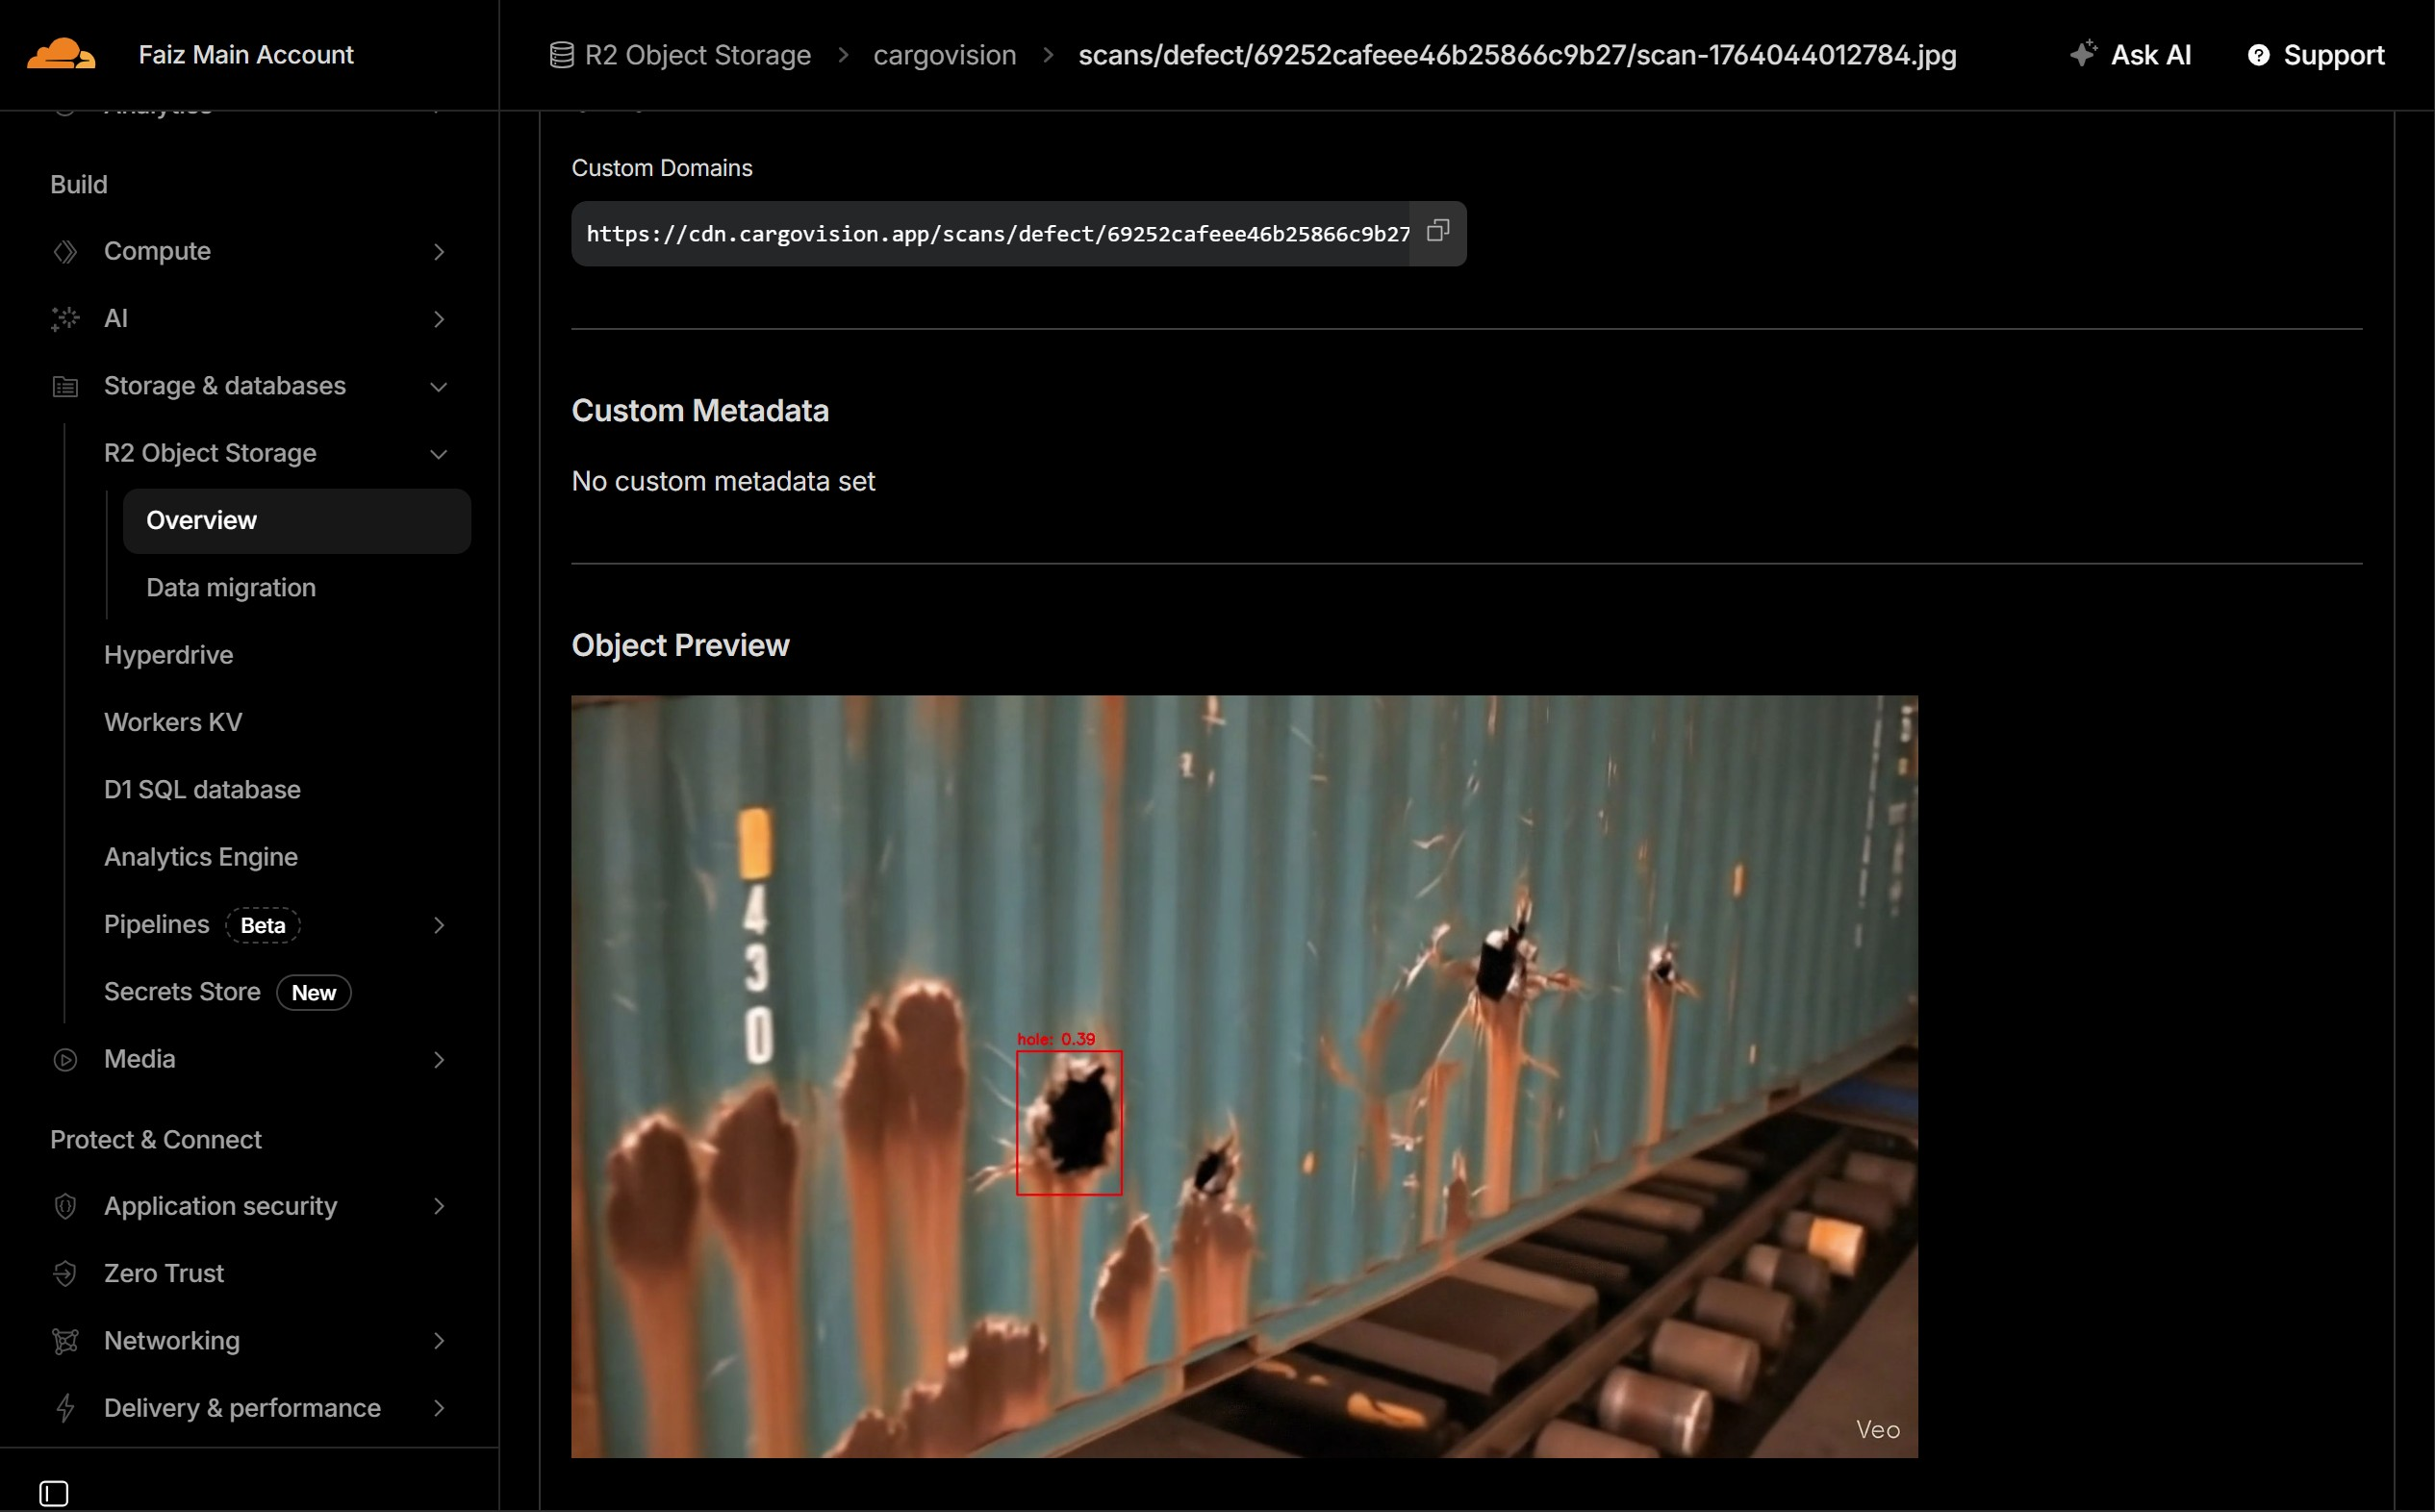
\includegraphics[width=0.78\textwidth]{images/evidence-r2-storage.jpg}
  \caption[Artefak visual pada Cloudflare R2]{Contoh penyimpanan artefak visual hasil pemindaian pada Cloudflare R2}
  \label{fig:evidence_r2_storage}
\end{figure}

Gambar~\ref{fig:evidence_r2_storage} menunjukkan bahwa artefak visual hasil
pemindaian benar-benar disimpan pada penyimpanan objek dan direferensikan
melalui alamat yang terpisah dari data transaksional. Bukti ini memperkuat
keputusan arsitektural untuk memisahkan data inti pada entitas kontainer dari
berkas visual berukuran besar agar riwayat kontainer tetap terjaga tanpa
membebani model data utama.
